\documentclass[hyperref={colorlinks=false},handout,10pt]{beamer}
\usetheme{Singapore} % Berlin
\usecolortheme{lily} %{wolverine} %lily
\usefonttheme[onlymath]{serif} % What does this do? 

\newcommand{\mygreen}{\color{green!50!black}}
\newcommand{\myblue}{\color{blue}}
\newcommand{\myred}{\color{red}}
\xdefinecolor{titlecolor}{rgb}{.855,.647,.125}
\setbeamercolor{frametitle}{fg=titlecolor}
\setbeamerfont{frametitle}{series=\bfseries}
%\setbeamerfont{headline}{size=\fontsize{9}{1}}
\setbeamercolor{math text}{fg=green!50!black} % Why is the math text greeen?? 
\setbeamercolor{normal text in math text}{parent=math text}

\setbeamertemplate{navigation symbols}{} %gets rid of navigation symbols
%\setbeamertemplate{mini frames}{}
\setbeamertemplate{footline}[frame number]
\beamertemplateshadingbackground{blue!5}{yellow!10}


\usepackage{graphicx}
\usepackage{tikz}
%\usepackage{handoutWithNotes}
%\pgfpagesuselayout{4 on 1 with notes}[a4paper,border shrink=2mm]

\usepackage{pgfpages}
\pgfpagesuselayout{4 on 1}[a4paper, border shrink=5mm, landscape]

\newlength{\wideitemsep}
\setlength{\wideitemsep}{\itemsep}
\addtolength{\wideitemsep}{100pt}
\let\olditem\item
\renewcommand{\item}{\setlength{\itemsep}{0.5\baselineskip}\olditem}


\def\LaTeXs{\LaTeX\ }

%\usetikzlibrary{calc,fadings,decorations.pathreplacing,backgrounds}
%% helper macros
%\tikzset{variable/.default=}  
%\tikzset{%
%    add/.style args={#1 and #2}{ to path={%
%    ($(\tikztostart)!-#1!(\tikztotarget)$)--($(\tikztotarget)!-#2!(\tikztostart)$)%
%\tikztonodes},add/.default={.2 and .2}}
%}  

%\tikzset{%
%    >=latex,
%    inner sep=0pt,
%    outer sep=2pt,
%    mark coordinate/.style={inner sep=0pt,outer sep=0pt,minimum size=2pt,
%    fill=black,circle}%
%}

\usepackage{textcomp}
\usepackage{listings}
\lstset{
basicstyle=\footnotesize\ttfamily,
language=R,
upquote=true,
breakatwhitespace=true,
columns=fullflexible,
keepspaces,
%numbers=none,
tabsize=3,
frame=bottomline,
framextopmargin=50pt,
showstringspaces=false,
extendedchars=true
}

\usepackage{amsmath,amsthm,amssymb}


\usepackage{float}
\floatstyle{boxed} % What does this do? 
\usepackage{mathpazo}
\usepackage{movie15}
\usepackage{bm}
%\usepackage{comment} % What does this do? 
\usepackage{caption}
\usepackage{subcaption}
\captionsetup[subfigure]{labelformat=empty}
\captionsetup[figure]{labelformat=empty}
\graphicspath{{./images/}}


\title{{\color{blue} \LARGE 550.400: Mathematical Modeling and Consulting\newline} }

\subtitle{{\color{red} \large Lecture Notes} }

\author{ 
    {\bf{Instructor:}} \\ 
Dr.~N.~H.~Lee \\ 
    \vspace{5pt}
} 
\institute{JHU AMS 2012 FALL}

\date{\mygreen Last Compiled on \today} 


\begin{document}

\begin{frame}[plain]
  \titlepage
\end{frame}

\begin{frame}%[shrink]
  \frametitle{Outline}
  \tableofcontents
\end{frame}

\section{FAQ} 

\begin{frame}
    \frametitle{What is that on the slide?}
    \begin{center}
        \Large
        \href{http://connect.johnshopkins.edu/welcome/}{http://connect.johnshopkins.edu/welcome/}
\end{center}
\end{frame}




\begin{frame}[fragile]
    \frametitle{How to add a figure in your work statement?}
        Note that \verb$<++>$ denotes a thing that you need to fill in.
        See the \texttt{lecture.tex} for (many) examples.
        \vskip0.1in
    \begin{lstlisting}
\begin{figure}
    \caption{<+caption text+>}
    \begin{center}
        \includegraphics[width=<++>\textwidth]{<++>}
    \end{center}
\end{figure}<++>
    \end{lstlisting}
\end{frame}

\begin{frame}
    \frametitle{Commit? Add? What is the difference?}
    \begin{block}{An imperfect analogy}
        \begin{itemize}
            \item Just like doing your HW with many questions
            \item For each question, first you do some work
            \item \texttt{git add} is like you being satisfied with your current
                version of your answer
            \item \texttt{git commit} is like you transcribing your solution to your
                paper that you will actually submit
            \item \texttt{git push} is like submitting your solution to the
                instructor so that they can see
        \end{itemize}
    \end{block}
\end{frame}

\begin{frame}
    \frametitle{Sorry \ldots but still confused about git \ldots}
    \begin{center}
        \href{http://gitref.org/index.html}{http://gitref.org/index.html}
    \end{center}
\end{frame}


\section{Git} 
\begin{frame}[allowframebreaks,fragile]
    \frametitle{Class Exercise}
    \begin{block}{Exercise 1}
    \begin{figure}
        \caption{\Large This is called a \emph{commit} graph}
        \begin{center}
            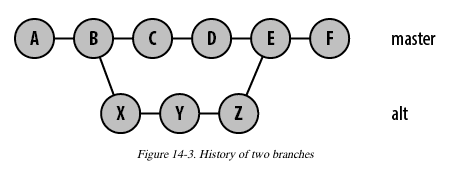
\includegraphics[width=\textwidth]{images/gitmergehistory.png}
        \end{center}
    \end{figure}
    \end{block}
    \vskip0.5in
    
    \begin{block}{Create a git folder with the following history}
         \begin{itemize}
             \item Each node's label signifies the commit 
             \item The folder contains only one single file \texttt{main.txt}
                 throughout the history
             \item Keep ``the story'' simple
             \item Push it to your github (remote) repository
         \end{itemize}
    \end{block}

    \begin{block}{Exercise 2}
        Collect all 8 stanzas of the ``Elephant'' poem from the course 
        github remote repositories and then push the resulting 
        one to \emph{your} github repository.
    \end{block}
    You will need the following addresses:
    \begin{lstlisting}
git://github.com/nhlee/550400.stanza1.git 
git://github.com/nhlee/550400.stanza2.git 
git://github.com/nhlee/550400.stanza3.git 
git://github.com/nhlee/550400.stanza4.git 
git://github.com/nhlee/550400.stanza5.git 
git://github.com/nhlee/550400.stanza6.git 
git://github.com/nhlee/550400.stanza7.git 
git://github.com/nhlee/550400.stanza8.git 
    \end{lstlisting}
\end{frame}


%\begin{frame}[allowframebreaks,fragile]
%    \frametitle{Adv. Git Method for Off-Line Teamwork}
%    \begin{figure}
%        \begin{center}
%            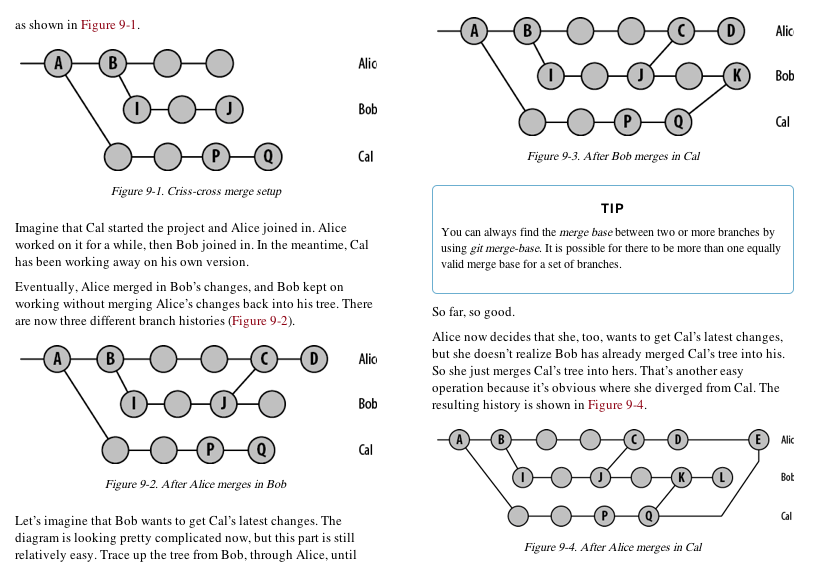
\includegraphics[width=0.8\textwidth]{images/gitmergeexample.png}
%        \end{center}
%    \end{figure}
%    \begin{lstlisting}
%git branch alice 
%git checkout alice
%git remote add altorigin git://git.com/do/not/copy/and/paste/this
%git push origin alice
%git branch -D alice
%    \end{lstlisting}
%
%    \begin{lstlisting}
%git format-patch master~2..master
%    \end{lstlisting}
%    \begin{figure}
%        \begin{center}
%            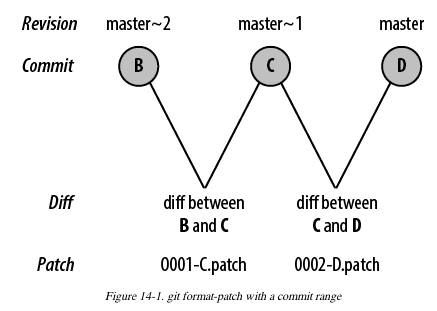
\includegraphics[width=0.7\textwidth]{images/gitformatpatch.png}
%        \end{center}
%    \end{figure}
%\end{frame}

\section{Causality \& Spurious Correlation}

\begin{frame}[allowframebreaks,fragile]
    \frametitle{Spurious Causality}

    \begin{lstlisting}
cbe.loc<-'http://www.massey.ac.nz/~pscowper/ts/cbe.dat';
cbe <- read.table(cbe.loc,header=T);
plot(cbe[,1],cbe[,3]);
    \end{lstlisting}

    \begin{lstlisting}
set.seed(10);
x <- rnorm(100);
y <- rnorm(100);
for(i in 2:100) {
    x[i] <- x[i-1] + rnorm(1);
    y[i] <- y[i-1] + rnorm(1);
}
plot(x,y);
    \end{lstlisting}
    \vskip0.5in

    \begin{lstlisting}
x <- y <- mu <- rep(0,1000);
for(i in 2:1000) mu[i] <- mu[i-1] + rnorm(1);
x <- mu + rnorm(1000);
y <- mu + rnorm(1000);

xrate.loc <-'http://www.massey.ac.nz/~pscowper/ts/us_rates.dat';
xrates <- read.table(xrate.loc,header=T);
plot(xrates$UK,xrates$EU,pch=4);
    \end{lstlisting}
    \vskip0.5in
    Then, how to detect the underlying factors? 
    \begin{lstlisting}
require(tseries)
adf.test(x)$p.value
adf.test(y)$p.value
po.test(cbind(x,y))

pp.test(xrates$UK)
pp.test(xrates$EU)
po.test(cbind(xrates$UK,xrates$EU))
ukeu.lm <- lm(xrates$UK ~ xrates$EU)
ukeu.res <- resid(ukeu.lm)
    \end{lstlisting}
\end{frame}

\begin{frame}
    \frametitle{Assessing Causality (527)}
    \begin{itemize}
        \item Consistency of association: 
            \begin{verse}
The association is observed in several different
populations using different types of study design. 
\end{verse}
        \item Strength of association
            \begin{verse}
A bigger difference in outcomes between cases with and without the purported
causal factor indicates a stronger association.
\end{verse}
        \item Temporal relationship
            \begin{verse}
The
cause preceded the effect. A correlation between two variables measured at the
same time gives weaker evidence than one measuring the relationship between
changes in the supposed cause and subsequent responses in the outcome. 
\end{verse}
        \item Mechanism
            \begin{verse}
There is a plausible means by which the alleged cause could affect
the outcome.
\end{verse}
    \end{itemize}
\end{frame}

\begin{frame}
    \frametitle{Writing about Causality (549)}
    \begin{block}{Vocab. Issues}
        \begin{verse}
           Carefully select the words you use to describe associations: verbs such as "affect" or "cause" and nouns such as "consequences" or "effects" all imply causality. "Correlated" or "associated" do not.
        \end{verse}
    \end{block}
   
    \begin{block}{Limits of Study Design}
        \begin{verse}
            \ldots it is much more difficult for one study to simultaneously
            show that all for criteria \emph{are} true.  \ldots For study
            designs that do not allow a cause-effect pattern to be tested
            well, point out those weaknesses and their implications for
            inferring causality; \ldots
        \end{verse}
    \end{block}
    
\end{frame}


\section{\LaTeX}
\begin{frame}[allowframebreaks,fragile]
    \frametitle{Intro.\ to work-statement template}
    \begin{lstlisting}
\documentclass[12pt,letterpaper][aritcle]
\usepackage{amsmath,amsthm,amssymb,amsfonts} # for popular math add-on
\usepackage{graphicx} # for inserting png, jpeg, pdf files as figure
\usepackage{bm} # for bold math
# some preamble stuff omitted (see the actual template)
\begin{document}
\section{A}
    \section{a}
        \paragraph{Hello World}
        \begin{align*}
            &f(x) = \int_0^1 \sin(u+x) du, \\
            &f(\bm x) = \int_0^1 \sin(u+\|\bm x\|) du.
        \end{align*}
\end{document}
    \end{lstlisting}
    
    
\end{frame}

\begin{frame}[allowframebreaks,fragile]
    \frametitle{Introduction to beamer}
    Basic Body Layer
    \begin{lstlisting}
\begin{document}
\section{Hello World} 
    \section{hello world}
        \begin{frame}
            \frametitle{hi world}
            \begin{columns}
                \begin{column}{0.5\textwidth}
                    \begin{itemize}
                        \item Alice!
                    \end{itemize}
                \end{column}
                \begin{column}{0.5\textwidth}
                    \begin{block}{hey world}
                        Bob!
                    \end{block}
                \end{column}
            \end{columns} 
        \end{frame}
\end{document}
    \end{lstlisting}
    Basic Preambles 
\begin{lstlisting}
\documentclass[hyperref={colorlinks=false},handout,10pt]{beamer}
\usetheme{Singapore}
\usecolortheme{lily}
\usefonttheme[onlymath]{serif} % What does this do? 
\end{lstlisting}    
    OR
\begin{lstlisting}
\documentclass[hyperref={colorlinks=false},handout,10pt]{beamer}
\usetheme{Berlin}
\usecolortheme{wolverine}
\usefonttheme[onlymath]{serif} % What does this do? 
\end{lstlisting}    
    For a more complete array of themes, go to: 
    \begin{center}
        \href{http://www.hartwork.org/beamer-theme-matrix/}{{http://www.hartwork.org/beamer-theme-matrix/}}
    \end{center}
SO, how to put a code in the slide? and it looks like codes? 
\begin{columns}
    \begin{column}{0.5\textwidth}
    \begin{verbatim}
\begin{lstlisting}
require(tikzDevice)
x = rnorm(100)
plot.ts(x)
dev.off()
\end{lstlisting}
    \end{verbatim}
    \end{column}
    \begin{column}{0.5\textwidth}
\begin{lstlisting}
require(tikzDevice)
x = rnorm(100)
plot.ts(x)
dev.off()
\end{lstlisting}
    \end{column}
\end{columns} 
But, this requires the following in the preamble portion 
of your tex file:
\begin{verbatim}
\usepackage{listings}
\lstset{
basicstyle=\footnotesize\ttfamily,
numbers=left,
frame=bottomline,
framextopmargin=50pt,
}
\end{verbatim}
Where to get more help:
\begin{center}
    \href{http://en.wikibooks.org/wiki/LaTeX/Presentations}{
    {http://en.wikibooks.org/wiki/LaTeX/Presentations}}
\end{center}
\end{frame}

\section{R \& Matlab}

\begin{frame}[fragile]
    \frametitle{How to do software documentation (via R)}
     \begin{lstlisting}
myfun <- function(x) {x^2} 
package.skeleton(name='MYPAC', 
                list='myfun',  
                path='~/')
#Do the documentation
system('R CMD check ~/MYPAC')
system('R CMD build ~/MYPAC')
system('R CMD install MYPAC')
     \end{lstlisting}
\end{frame}

\begin{frame}[fragile,allowframebreaks]
    \frametitle{Using R to do System Admin Stuff}
    \begin{lstlisting}
for(itr in 1:8) {
    stanzaname = paste("stanza",itr,sep="")
    gitaddress = paste("git://github.com/nhlee/550400.",
                            stanzaname,".git",sep="")
    bashcommand = paste("git remote add ",
                            stanzaname," ",gitaddress,sep="")
    system(bashcommand)
}
    \end{lstlisting}
    \begin{itemize}
        \item \texttt{1:8} creates a vector that \ldots 
        \item \texttt{X = 1} assigns 1 to X 
        \item \texttt{X <- 1} also assigns 1 to X
        \item lots of things are done through function 
        \item \texttt{paste} and \texttt{system} are functions that \ldots 
        \item functions has none or more arguments 
        \item arguments are implicitly ordered but the order can be overridden
    \end{itemize}
    \begin{lstlisting}
system(`ls -ld .*')
system(`cat .Rprofile')
system(`cat .bashrc')
system(`cat .gitignore')
system(`cat .vimrc')
    \end{lstlisting}
    \begin{itemize}
        \item .xxx files are hidden
        \item ls -ld .* show the hidden files
        \item .Rprofile set up your R behavior
        \item .bashrc set up your bash behavior
        \item .gitignore set up your git behavior 
        \item .vimrc set up you vim behavior
        \item these files are equivalent to Preference part of your GUI
            software
    \end{itemize}
\end{frame}




\section{Vim for efficient editing}
\begin{frame}
    \frametitle{FAQ}
    \begin{itemize}
        \item How to start vim? 
        \item How to quite vim?
        \item 
    \end{itemize}
\end{frame}<++>
\begin{frame}
    \frametitle{Vim for efficient editing}
    \begin{block}
        {Vim is a \emph{highly customizable} text editor}
    \vskip0.1in
    \begin{enumerate}
        \item \LaTeX, R, C/C++, Java, Python, Git and etc.
        \item Regular expression, syntax coloring, auto-completion
        \item \texttt{<ESC>}-mode
        \begin{itemize}
            \item \texttt{:}-mode, aka., the last line mode
            \item \texttt{i}-mode, aka., the insert mode
        \end{itemize}
    \end{enumerate}
    \end{block}
\end{frame}

\begin{frame}
    \frametitle{Vim for efficient editing}
    \begin{itemize}
        \item Download \& Install GVim or MacVim
        \item Download \& Install tetris.vim
        \item Download \& Install minibufexpl.vim
        \item Download \& Install Gundo 
        \item Download \& Install Vim-LaTeX
    \end{itemize}
\end{frame}

\begin{frame}
    \frametitle{Vim for efficient editing}
    \begin{figure}
        \begin{center}
            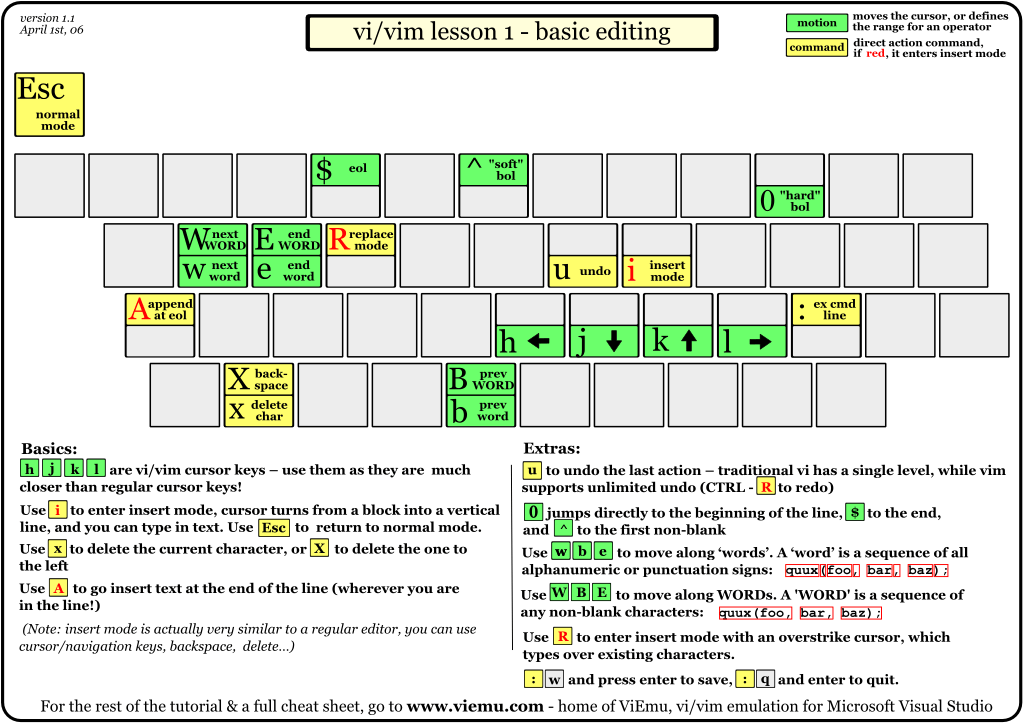
\includegraphics[width=\textwidth]{images/vi-vim-tutorial-1.png}
        \end{center}
    \end{figure}
\end{frame}

\section{Math Modeling}

\begin{frame}
    \frametitle{A Word Problem}
    \begin{verse} 
        To encourage Elmer's promising tennis career, his father offers him a
        prize if he wins (at least) two tennis sets in a row in a three-set
        series to be played with his father and the club  champion
        alternately: father-champion-father or champion-father-champion,
        according to Elmer's choice. The champion is a better player than
        Elmer's father. Which series should Elmer choose?
    \end{verse}
  \vskip0.1in
  \begin{itemize}
      \item What is that you wish to know?
      \item unimportant, exogenous, and endogenous?
      \item if the model fits the situation, will we be able to use it? 
      \item Test the model
  \end{itemize}
\end{frame}

\begin{frame}[allowframebreaks]
    \frametitle{Arguments from Scale}
    \begin{block} {Cost of Packing}

    \end{block}
    \begin{block}{Speed of Racing Shells}
        
    \end{block}
    \begin{block}{Size Effect in Animal}
        
    \end{block}
\end{frame}


%\section{Class Info.}
\begin{frame}
    \frametitle{Syllabus}
    \begin{itemize}
        \item Grade Policy
        \item Attendance
        \item \emph{Tentative} Schedule
        \item Blackboard
        \item Misc.
    \end{itemize}
\end{frame}

\begin{frame}
    \frametitle{OH Location}
    \begin{figure}
        \caption{Clark Hall 320B}
        \begin{center}
            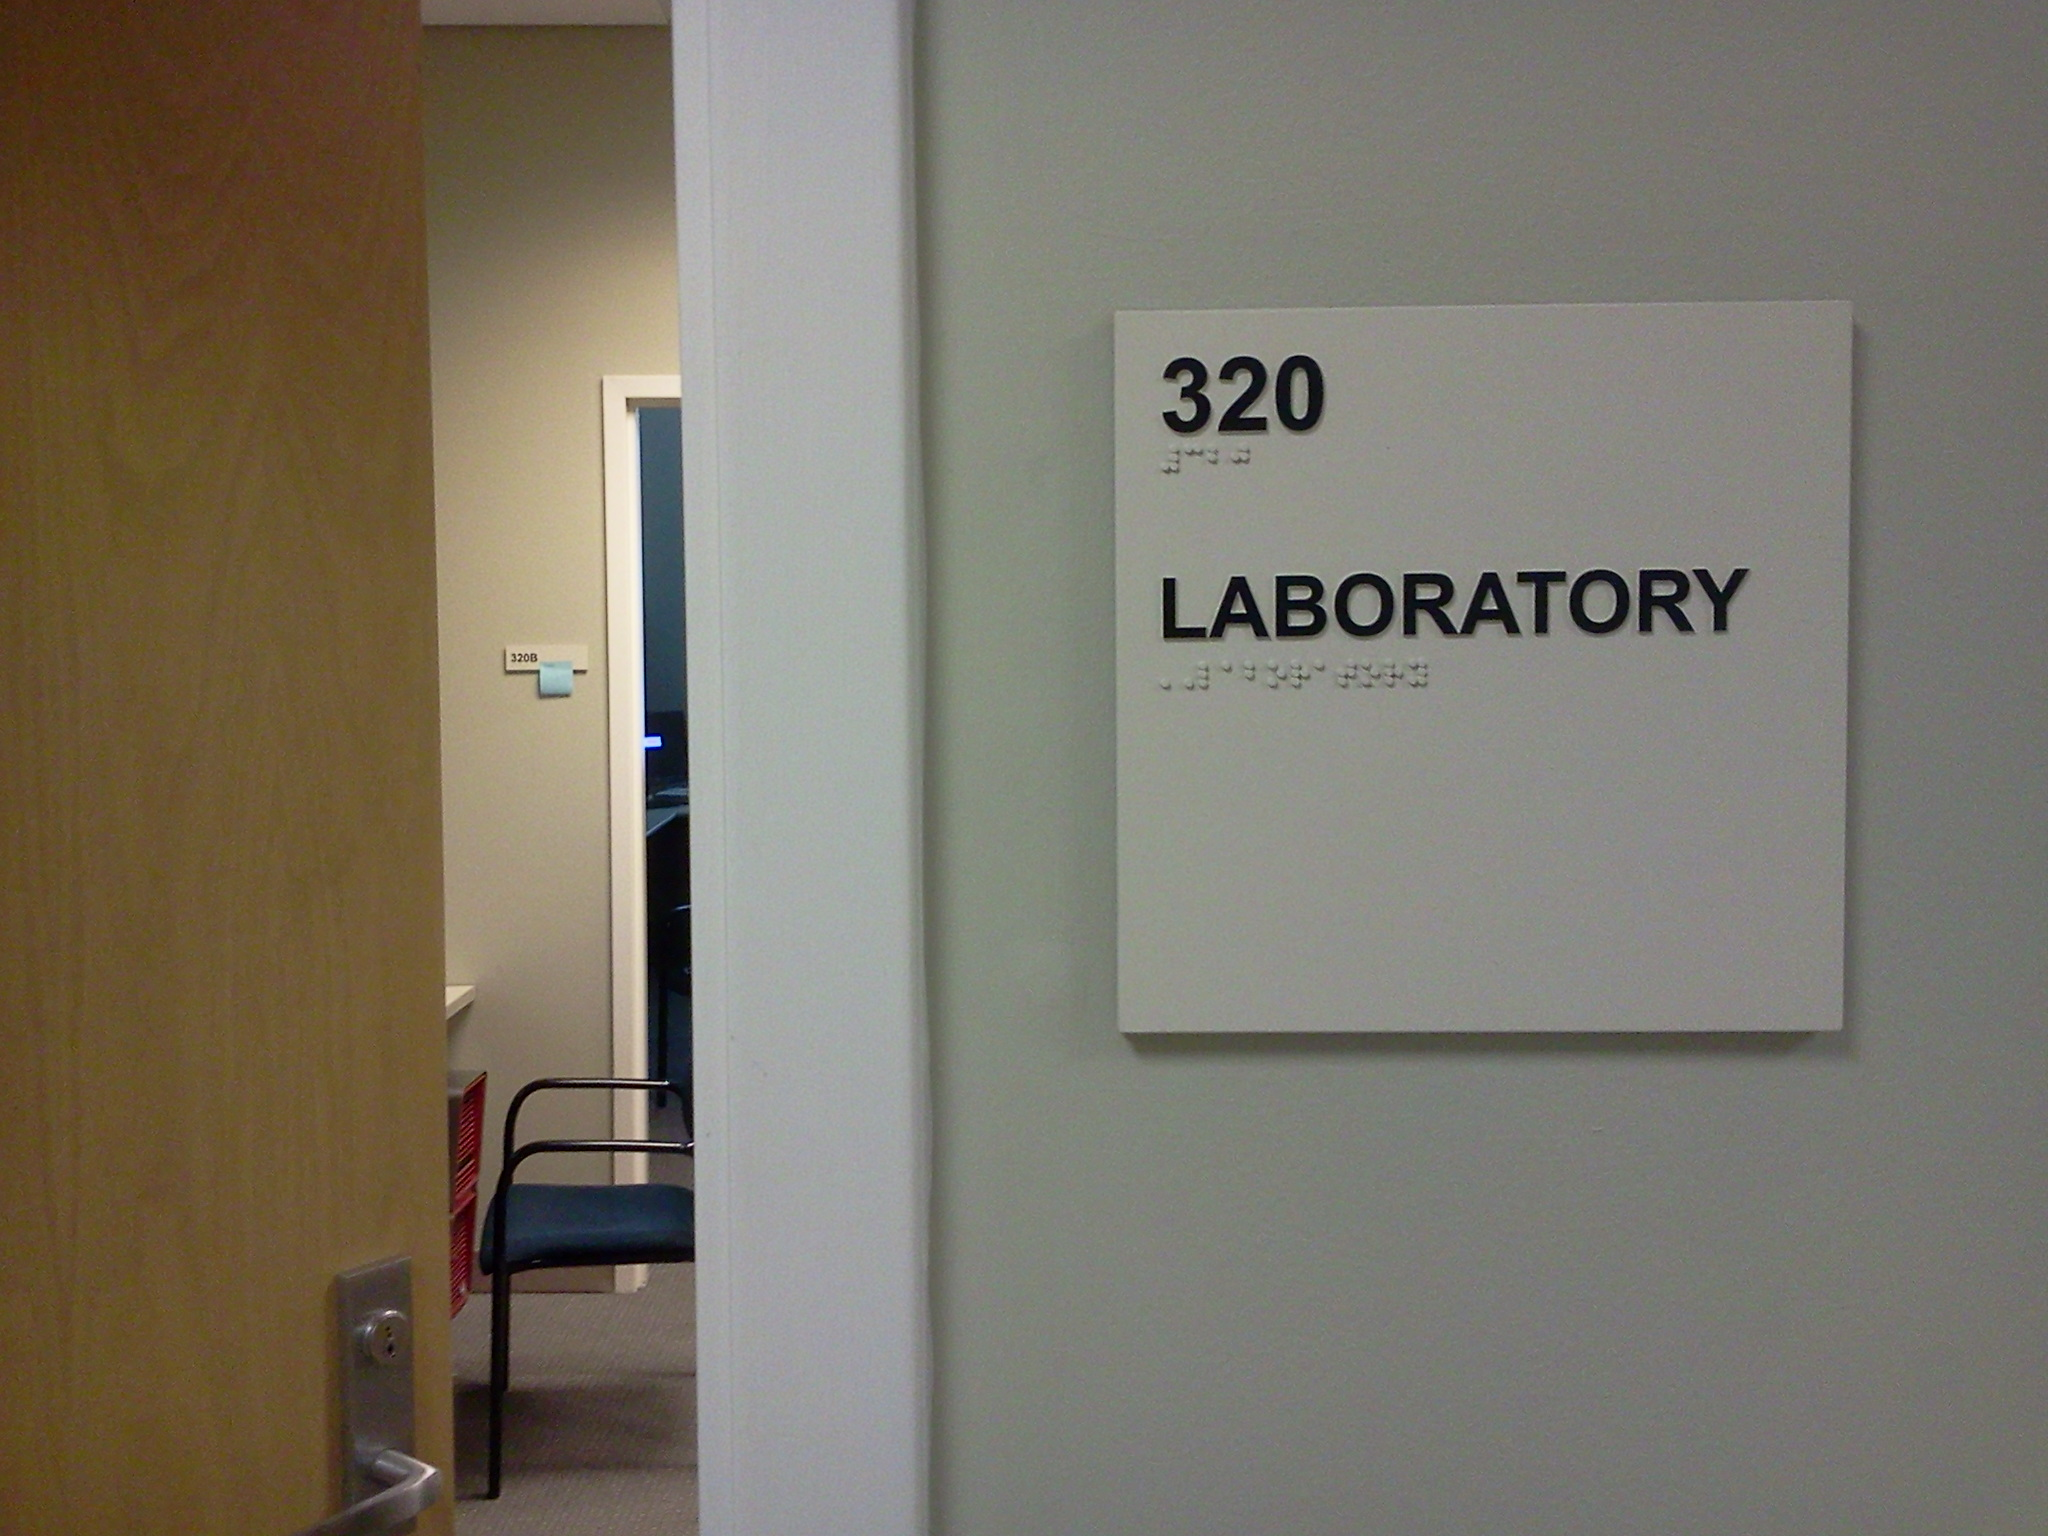
\includegraphics[width=0.75\textwidth]{images/Clark320B.jpg}
        \end{center}
        \label{fig:ClarkHall320B}
    \end{figure}
\end{frame}

\begin{frame}[fragile]
    \frametitle{Course Book Reserve}
    \vskip0.5in
    \begin{center}
        \href{https://catalyst.library.jhu.edu/reserves/13812}{JHU Library Reserve Service}
    \end{center}
\end{frame}

\begin{frame}
    \frametitle{Presentations in this class}
    \begin{figure}
        \caption{For your presentation recording needs}
        \href{https://know.it.jhu.edu/display/TECHCLASS/Homewood+Campus}{
        
\includegraphics[width=0.7\textwidth]{images/BLC2006.jpg}}
    \end{figure}
\end{frame}

\begin{frame}[fragile]
    \frametitle{Unofficial Way to Access the Course Folder}
    \vskip0.5in
    \begin{center}
        \href{http://cis.jhu.edu/~nhlee/550400.html/}{
            \url{http://cis.jhu.edu/~nhlee/550400.html/}
        }
    \end{center}
\end{frame}


%\section{Textbook Materials}

\subsection{Writing about Numbers}

\begin{frame}
    \frametitle{Outline}
    \tableofcontents[currentsection, currentsubsection]
\end{frame}
\begin{frame}
    \frametitle{Seven Basic Principles}
     \begin{enumerate}
         \item Set the context 
         \item Choose effective examples and analogies
         \item Choose vocabulary to suit your readers
         \item Decide whether to present \#s in text, tables, or figures
         \item Report and interpret \#s in the text
         \item Specify the direction \emph{and} size of an association between variables
         \item For many \#s, summarize overall pattern 
     \end{enumerate}
\end{frame}

\begin{frame}
    \frametitle{WMA Problem 2.5a \& 2.6a}
        \begin{verse}
            The Williams family's income of \$25,000 falls below 185\% of the 
            \href{http://aspe.hhs.gov/poverty/12poverty.shtml}{Federal Poverty
            Threshold} for a family of four, qualifying them
            for food stamps. 
        \end{verse}
        \vskip0.3in
\begin{description}
    \item[Problem 2.5a] {Identify terms that need to be defined or restated
        for a nontechnical audience}
    \item[Problem 2.6a] Rewrite the sentences in the previous questions for an
        audience with a fifth-grade education.  Convey the main point,
        not the calculation or the jargon. 
    \item[FYI] \href{http://www.bloomberg.com/video/how-the-rich-get-richer-and-the-poor-poorer-kfuILNN9SoaQXLd5cVBwPQ.html}{Off-the-chart}
\end{description}
        
\end{frame}

\begin{frame}
    \frametitle{WMA Problem 2.8a}
    Rewrite each of these sentences to specify the direction and magnitude of
    the association:
    \vskip0.1in
    \begin{center}
    \begin{verse}
        In the United States, race is correlated with income. 
    \end{verse}
    \end{center}
    \begin{table}
        \centering
        \caption{\textbf{Median income by race and Hispanic origin, United States, 1999}}
        \label{tab:WMAex2x8}
        \begin{tabular}{lc}
        Race/Hispanic origin & Median Income \\
        \hline 
        White   & \$42,504 \\
        Black   & \$27,910 \\ 
        Asian/Pacific Islander   & \$51,205 \\ 
        Hispanic (can be of any race) & \$30,735 \\
        \hline
        \end{tabular}
    \end{table}
\end{frame}

\begin{frame}
    \frametitle{WMA Problem 2.9}
    Use the GEE approach to describe the patterns in the figure below,
    including an introductory sentence about the purpose of the chart 
    before summarizing the patterns. 
    \begin{figure}
        \begin{center}
            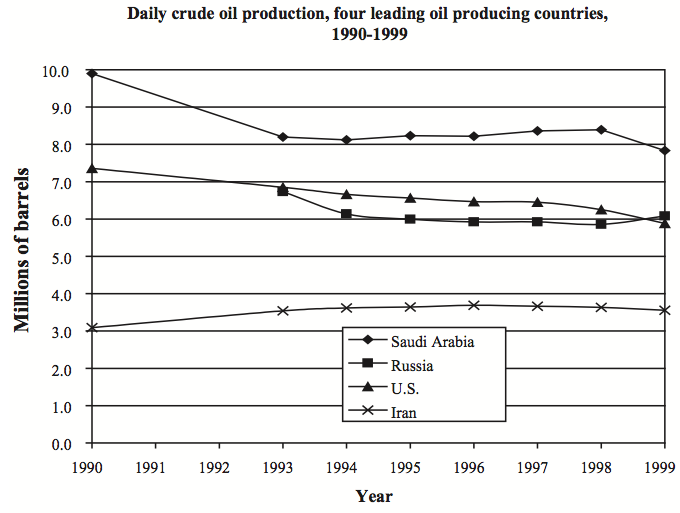
\includegraphics[width=0.6\textwidth]{images/WMAex2x9.png}
        \end{center}
    \end{figure}
\end{frame}

\subsection{Math. Modeling}


\begin{frame}
    \frametitle{Outline}
    \tableofcontents[currentsection, currentsubsection]
\end{frame}

\begin{frame}
    \frametitle{Models and Reality: ``Disclaimer''}
    \begin{verse}
        Here we are concerned exclusively with mathematical models, that is,
        models that mimic reality by using the language of mathematics.
        Whenever we use ``model'' without a modifier, we mean ``mathematical
        model.''
    \end{verse}
\end{frame}

\begin{frame}
    \frametitle{Models and Reality}
    \begin{verse}
    What makes Mathematical models useful? 
    If we ``speak in mathematics,'', 
    \begin{itemize}
        \item We must formulate our ideas precisely and so are less likely to
            let implicit assumptions slip by,
        \item We have a concise ``language'' which encourages manipulation,
        \item We have a large number of potential theorems available,
        \item We have high speed computers available for carrying out calculations.
    \end{itemize}
    \end{verse}
\end{frame}

\begin{frame}
    \frametitle{Properties of Models}
    \begin{verse}
        A mathematical model is an abstract, simplified, mathematical
        construct related to a part of reality and created for a particular
        purpose.
    \end{verse} 
    \begin{verse} 
        Since a dozen different people are likely to come up with a
        dozen different definitions, don't take this one too seriously;
    \end{verse}
    \begin{verse}
        rather, think of it as a crude starting point around which to build
        your own understanding of mathematical modeling.
    \end{verse}
\end{frame}

\begin{frame}
    \frametitle{Properties of Models}
    \begin{verse}
    As far as a model is concerned, the world can be divided into three parts:
    \begin{enumerate}
        \item Things whose effects are neglected,
        \item Things that affect the model but whose behavior the model is not
            designed to study,
        \item Things the model is designed to study the behavior of. 
    \end{enumerate}
\end{verse}
\end{frame}

\begin{frame}
    \frametitle{Building a Model: ``Disclaimer''}
    \begin{verse}
        Model building involves imagination and skill. Giving rules for doing
        it is like listing rules for being an artist; at best this provides a
        framework around which to build skills and develop imagination. 
    \end{verse} 
    \begin{verse}
        It may
        be impossible to teach imagination. I won't try, but I hope this book
        provides an opportunity for your skills and imagination to grow. With
        these warnings, I present an outline of the modeling process.
    \end{verse}
\end{frame}


\begin{frame}
    \frametitle{Building a Model}
    \begin{verse}
        With these warnings, I present an outline of the modeling process.
    \begin{description}
        \item[1.] {Formulate a problem}
        \item[2.] {Outline the model}
        \item[3.] {Is it Useful?}
        \item[3.] {Test the model}
    \end{description}
    \end{verse}
\end{frame}

\begin{frame}
    \frametitle{Building a Model}
    \begin{verse}
        Some models may require no data. If a model makes the same prediction
        regardless of the data, we are not getting something for nothing because
        this prediction is based on the assumptions of the model. 
    \end{verse}
   
    \begin{verse}
        To some extent,
        the distinction between data and assumptions is artificial. In an extreme
        case, a model may be so specialized that its data are all built into the
        assumptions.
    \end{verse}
\end{frame}

\begin{frame}
    \frametitle{Building a Model}
    \begin{verse}
        The manager of a large commercial printing company 
        asks your advice on how many salespeople to employ.  
    \end{verse}
    \begin{verse}
        Qualitatively, more salespeople will increase sales overhead,
        while fewer salespeople may mean losing potential customers. 
    \end{verse}
    \begin{verse}
       Thus there should be some optimum number.
    \end{verse}
    
\end{frame}


\begin{frame}
    \frametitle{IMM Problem: ``Disclaimer''}
    \begin{verse}
        Some of the problems in this book lead you step by step through the
        development of a model and thus resemble the mathematics problems you have
        seen in other courses; 
    \end{verse} 
    \begin{verse} 
        however, many problems are closer to real life:
        They are vaguely stated, have multiple answers (models), or are open
        ended. 
    \end{verse}
    \begin{verse}
        I strongly recommend working in small groups on the problems to
        bring out various ideas and evaluate them critically.
    \end{verse}
\end{frame}

\begin{frame}
    \frametitle{IMM Problem 1.1}
    Suppose people enter the elevators in a skyscraper at random during the
    morning rush. The result will be several elevators stopping on each floor
    to discharge one or two passengers each. 
    \vskip0.1in
    \begin{itemize}
        \item Discuss schemes for improving the situation. 
        \item How could improvement be measured? 
        \item How could you model the situation to decide what scheme to adopt?
    \end{itemize}
\end{frame}

\begin{frame}
    \frametitle{IMM Problem 1.6}
    Unless you have been extremely lucky, you have had a large class in a
    poorly designed lecture hall. 
    
    \vskip0.25in
    \begin{description}
        \item[(a)] What are some criteria to be considered
    in designing a large lecture hall? 
    \end{description}
\end{frame}
    
\begin{frame}
    \frametitle{IMM Problem 1.6}
    Unless you have been extremely lucky, you have had a large class in a
    poorly designed lecture hall. 
    \vskip0.15in
    \begin{description}
        \item[(b)] One criterion is legibility of material written on the boards. 
        \begin{itemize}
            \item Construct a model of legibility as a function of 
                \begin{itemize}
                    \item  \emph{the distance} your seat is from the board 
                    \item \emph{the angle} at which you look at the board 
                \end{itemize}
            \item What will the curves of constant legibility look like on a
                floor plan?
            \item How can you test this prediction? Try it. 
            \item Does this suggest shaping the back of the hall differently
                than is usually done? How?
        \end{itemize}    
    \end{description}
    \vfill
\end{frame}
     
\begin{frame}
    \frametitle{IMM Problem 1.6}
    Unless you have been extremely lucky, you have had a large class in a
    poorly designed lecture hall. 
    
    \vskip0.25in
    \begin{description}
        \item[(c)] Can mathematical modeling help with any other criteria
    besides the one mentioned in (b)? Try to pick a criterion from among these
    possibilities and develop a model for it.
    \end{description}
\end{frame}
     
\begin{frame}
    \frametitle{Models and Reality}
    \begin{verse}
        The ultimate test of a model is how well it performs when 
        it is applied to the problem it was designed to handle.
    \end{verse}
    \vskip0.5in
    \begin{verse}
       A model is used, it may lead to incorrect predictions. The model is
       often modified, frequently discarded, and sometimes used anyway because
       it is better than nothing. This is the way science develops.  
    \end{verse}
\end{frame}




\section{Course Project}

\begin{frame}
    \frametitle{Outline}
    \tableofcontents[currentsection, currentsubsection]
\end{frame}


\begin{frame}[fragile]
    \frametitle{Mission Impossible?: an analogy}
    \begin{figure}
        \caption{Mission Impossible Season 2 Episode (00:00 -- 06:25)}
    \begin{center}
    \href{http://movies.netflix.com/WiPlayer?movieid=70157337&trkid=4431095&pt_request_id=a8a7108c-c068-4d22-b649-0b7095279045-1882594&pt_rank=4&pt_row=-1&pt_location=WATCHNOW#MovieId=70157337&EpisodeMovieId=70156671}{
            
\includegraphics[width=0.8\textwidth]{images/IMFproblemstatement.png}
    }
    \end{center}
    \end{figure}
\end{frame}

\begin{frame}
    \frametitle{Project in Industry: Frequently Recurring Elements}
    A stylized timeline:
    \vspace{7pt}
             \begin{enumerate}
                 \item Work Statement,
                 \item Midterm Presentation,
                 \item Progress Report,
                 \item Final Presentation,
                 \item Final Report.
             \end{enumerate}
    \begin{center}
        \href{http://www.ipam.ucla.edu/programs/rips2011/}{
        
\includegraphics[width=0.5\textwidth]{images/ipam}}        
    \end{center}
\end{frame}

\subsection{Work Statement}

\begin{frame}
    \frametitle{Outline}
    \tableofcontents[currentsection, currentsubsection]
\end{frame}

\begin{frame}
    \frametitle{What is Work Statement}
This is the written proposal and definition of the project and constitutes the
team's ``contract'' with the sponsor. It should be approximately 2-5 pages
long.  It sets forth the nature of the project, the specific
objectives of the project, the results expected, and the ``deliverables'' for
the project. The scope of the project must be within the timetable for the
program and that the deliverables are reasonable and appropriate; given the
nature of research, it should not include promises that the team cannot be
certain to achieve. It is ultimately given to the sponsor for review and
signature.
\end{frame}


\begin{frame}
    \frametitle{Template 1}
    \begin{enumerate}
        \item Abstract
        \item Background
        \item Problem description
        \item Approach (``time permitting'' clause for some work)
        \item Schedule (dates for completing milestones and tasks and for
            deliverables)
        \item Milestones (major checkpoints your team will use to stay on
            track)
        \item Deliverables (specific work products you will deliver to the
            sponsor)
    \end{enumerate}
\end{frame}

\begin{frame}
    \frametitle{Templates 2}
    \begin{enumerate}
        \item Introduction
        \item Problem background
        \item Mathematical background
        \item Computing background 
        \item Possible solutions and project objectives
        \item Deliverables (``time permitting'' clause for some work)
        \item Timeline
    \end{enumerate}
\end{frame}

\begin{frame}
    \frametitle{Template 3}
    \begin{enumerate}
        \item Project background
        \item Goals (major direction you see the work aimed at, not
            necessarily what you bid to do)
        \item Proposed mathematical approach
        \item Objectives (specific aims of your project, and schedule of
            results you expect to achieve)
        \item Optional objectives 
        \item Deliverables
        \item Milestones
        \item Work flowchart
        \item Schedule
    \end{enumerate}
\end{frame}

\begin{frame}
    \frametitle{Template 4}
    \begin{enumerate}
        \item Abstract
        \item Problem background
        \item Problem description
        \item Approach 
        \item Deliverables
        \item Timetable
        \item Team members
    \end{enumerate}
\end{frame}

\begin{frame}
    \frametitle{Work Statement}
    \begin{block}
        {In the initial segment (``Abstract'', ``Introduction'', ``Background'')}
        \begin{itemize}
            \item Brief description of the company
            \item Major product lines(s)
            \item A brief (abstract) description of the project
        \end{itemize}
    \end{block}
\end{frame}

\begin{frame}
    \frametitle{Work Statement}
    \begin{block}
        {Throughout}
        \begin{itemize}
            \item Spell out terminology -- avoid undefined jargon or acronym
            \item When options must be resolved, give dates by which they must
                be resolved
            \item Give modest objectives, not boastful ones
        \end{itemize}
    \end{block}
\end{frame}

\begin{frame}
    \frametitle{Work Statement}
    \begin{block}
        {List of deliverables should include}
        \begin{itemize}
            \item Site visits (to be arranged)
            \item Midterm oral presentation
            \item Midterm report
            \item Final presentation
            \item Final report
            \item Software (if appropriate) 
                \begin{itemize}
                    \item Specify sponsor-approved OS, platform
                    \item Documentations
                \end{itemize}
        \end{itemize}
    \end{block}
\end{frame}

\begin{frame}[allowframebreaks]
    \frametitle{Glossary}
    \begin{block}
        {GOAL} The overall, long range, end result that your research is aimed at, what
you are trying to achieve ultimately. Stating a goal does not mean you believe
you will get there this time around. It is the grand view towards which you
strive. The goal of AIDS research is to find a cure for AIDS.
\end{block}
\end{frame}

\begin{frame}
    \frametitle{Glossary}
    \begin{block}
        {OBJECTIVES} The specific things you will try to achieve in your project, the
immediate targets of your research. Your objectives spell out how you have
parsed the problem of heading towards the goal into smaller pieces that you
will work on. The objectives set practical limits on your work. They point to
where the project can reasonably expect to wind up. It should be clear that
the objectives fit into and work towards the long-range goal.
\end{block}
\end{frame}

\begin{frame}
    \frametitle{Glossary}
\begin{block}
        {TASKS} These are the specific things you will do in order to achieve your
objectives. The tasks drive your determination of what skills and other
resources (such as data, software, hardware, written materials, work
environment) will be needed for your project. If among the resources needed
are ones that must be supplied by the sponsor, then you will need to specify
these items in your Work Statement.
\end{block}
    
\end{frame}


\begin{frame}
    \frametitle{Glossary}
\begin{block}
        {DELIVERABLES} The things you promise to deliver to the sponsor. For a 
project, these include a mid-term and final report, a mid-term presentation
and a final presentation on Projects Day. They may also include site visits to
the sponsor (usually one near the beginning of the project to get acquainted
with the sponsor, and one after Projects Day to present the work at the
sponsor's location), software, perhaps hardware in some cases, written results
of literature searches, white papers (i.e., written background information on
such things as plans, methods or concepts prepared for internal use), etc.
These additional items are to be decided by you in consultation with your
sponsor’s mentor.
\end{block}
    
\end{frame}

\begin{frame}
    \frametitle{Glossary}
\begin{block}
        {MILESTONES} A list of specific accomplishments that you may use to mark
progress and maintain pace and coordination within your project. They are used
to help your team stay on track and to determine the success of a chosen line
of attack on your problem. Milestones may or may not be included in your Work
Statement, but you should definitely think these through for your own use as
you plan your project and Work Statement. They are check-points for you (and
for your sponsor, if they are included in the Work Statement), not necessarily
deliverables. You may want to specify major milestones in your Work Statements
to indicate what you would do if your research leads 
to the conclusion that some objective cannot be accomplished. For example, "if
by such a date we have found it impossible to achieve X, then we will begin
Y." Research is exploration of the unknown, so you may encounter an
intractable obstacle and need to work around it. You can't know everything
ahead of time. Give some thought to this and try to allow for milestones by
which you can judge where you are and what you need to do to proceed
effectively in the event you don't meet a milestone.
\end{block}
    
\end{frame}

\begin{frame}
    \frametitle{Glossary}
\begin{block}
        {SCHEDULE} This specifies when you will finish major parts of your research and
provides a timetable for completion of deliverables. Internally, you should
maintain as fine-grained a schedule as you need to keep your team coordinated
and on track, but in your Work Statement it is best to make the schedule and
list of deliverables as modest as the sponsor will allow.
\end{block}
    
\end{frame}

%\section{Example}

\subsection{Random Bits}

\begin{frame}
    \frametitle{Outline}
    \tableofcontents[currentsection, currentsubsection]
\end{frame}

\begin{frame}
    \frametitle{What is Mathematical Modeling?}
    \begin{figure}
            \centering
            \caption{
            \href{http://www.youtube.com/watch?feature=endscreen&v=UuXwYZ3AQU0&NR=1}
            {Money Ball}}
            \href{http://www.youtube.com/watch?v=WNlCBy07z08}{
            
\includegraphics[width=0.4\textwidth]{Moneyballs.jpg}
            }
            \label{fig:MondayBall} 
    \end{figure}
\end{frame}

\begin{frame}
    \frametitle{What is Mathematical Modeling?}
    \begin{figure}
        \centering
        \caption{
        \href{http://www.youtube.com/watch?v=Jzl39jqZjsw&feature=share&list=UUEWRMyobsgQG-PaC9ldME4A}{
        Trillion Dollar} 
        \href{http://www.youtube.com/watch?v=G17rx7H3DtI&feature=BFa&list=UUEWRMyobsgQG-PaC9ldME4A}{Bet}
        }
        \href{http://www.youtube.com/watch?v=dsrOXJwGwtk}{
        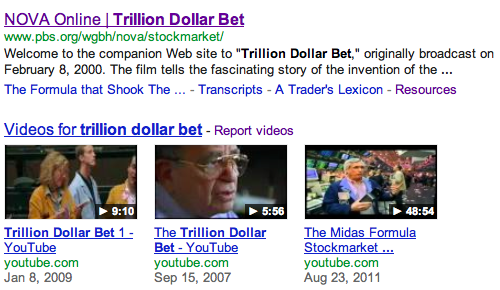
\includegraphics[width=\textwidth]{TrillionDollarBet.png}
        }
        \label{fig:LTCM}
    \end{figure}
\end{frame}

\begin{frame}
    \frametitle{What is Mathematical Modeling?}
    \begin{figure}
        \centering
        \caption{{LAPD Fighting Crime with Math}}
        \href{http://www.youtube.com/watch?v=HZ7fLuO7zb4}{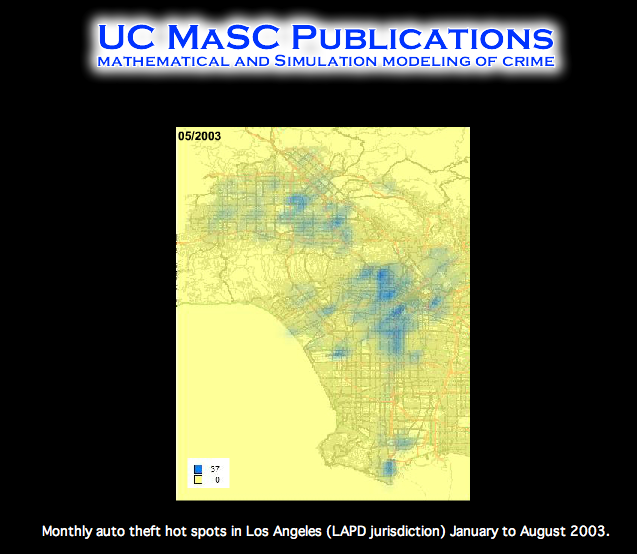
\includegraphics[width=0.6\textwidth]{LAPDUCLA.png}}
        \label{fig:LAPDUCLA}
    \end{figure}
\end{frame}

\begin{frame}[fragile]
    \frametitle{What is Mathematical Modeling?}
        \begin{figure}
            \centering
            \caption{Crime rates and religious beliefs}
            \href{http://www.economist.com/blogs/graphicdetail/2012/09/daily-chart/}{
            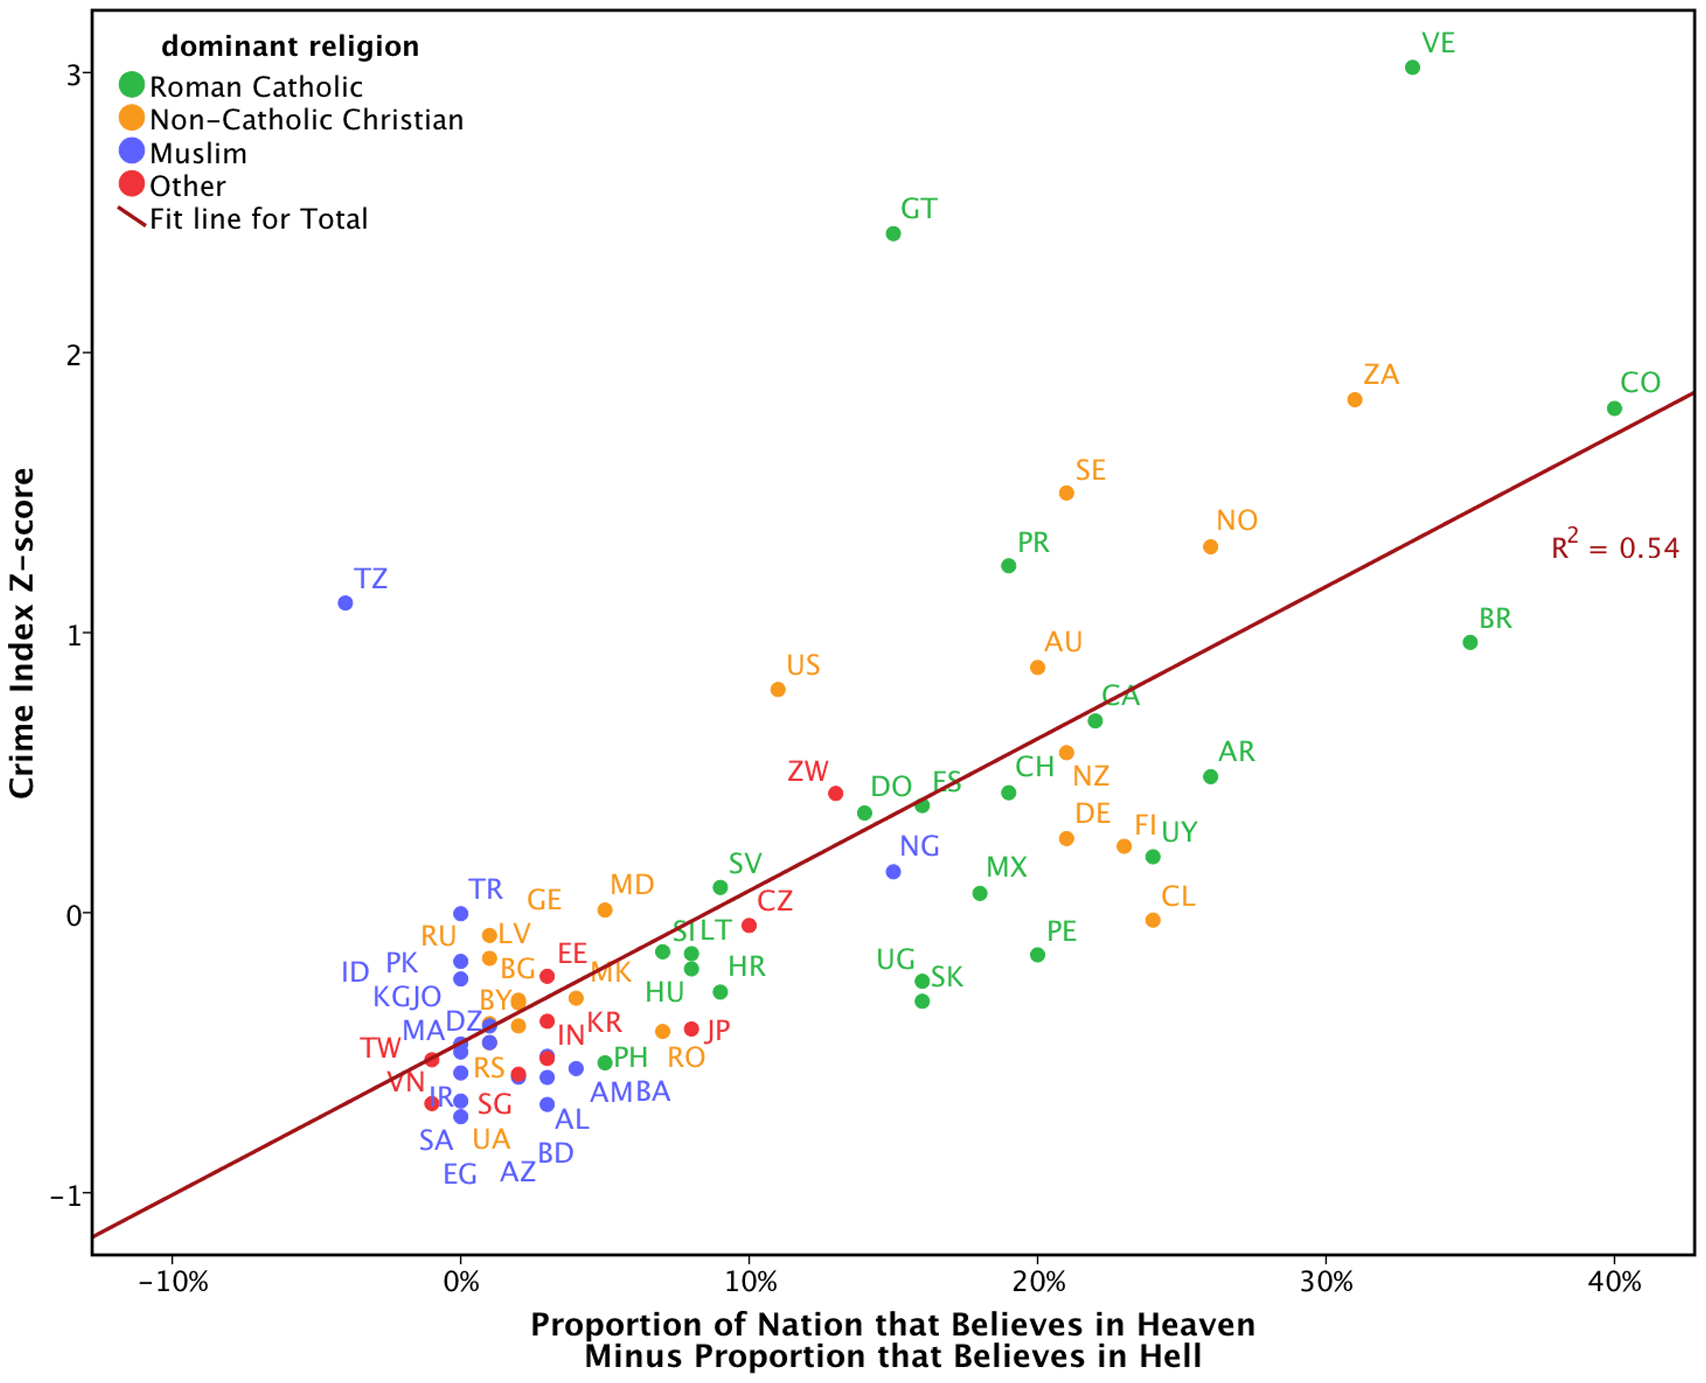
\includegraphics[width=0.7\textwidth]{images/hellvsheaven.png}}
    \end{figure}
\end{frame}

\begin{frame}[fragile]
    \frametitle{More Project Ideas}
    \begin{center}
    \href{http://www.stat.berkeley.edu/users/statlabs/}{http://www.stat.berkeley.edu/}
    \end{center}
    \vskip0.25in
    \begin{center}
        \href{http://www.math.msu.edu/Academic%5FPrograms/graduate/msim//ProjectPage.aspx}{http://www.math.msu.edu/}
    \end{center}
    \vskip0.25in
    \begin{center}
        \href{http://www.mathgoespop.com/2011/09/moneyball.html}{http://www.mathgoespop.com/}
    \end{center}
    \vskip0.25in
    \begin{center}
        \href{http://www.math.hmc.edu/clinic/projects/years/}{http://www.math.hmc.edu/clinic/}
    \end{center}
\end{frame}

\subsection{Insurance Redlining}

\begin{frame}
    \frametitle{Outline}
    \tableofcontents[currentsection, currentsubsection]
\end{frame}

\newtheorem{DEFinsredlining}{Insurance Redlining}
\newtheorem{DEFfairplan}{FAIR}
\begin{frame}
    \frametitle{ Insurance Redlining}
    \begin{DEFinsredlining}
        \textcolor{red}{Insurance redlining} refers to the practice of refusing
        to issue insurance to certain types of people or within some 
        geographic area. 
    \end{DEFinsredlining}
\vskip.5in
    \begin{DEFfairplan}
        The \textcolor{red}{FAIR} plan was offered by the city of Chicago as a 
        default policy to homeowner who had been rejected by the voluntary
        market. 
    \end{DEFfairplan}
\end{frame}

\begin{frame}
    \frametitle{ Insurance Redlining}
    \begin{figure}
        \centering
        \caption{Insurance Redlining}
        \href{http://en.wikipedia.org/wiki/Redlining}{
        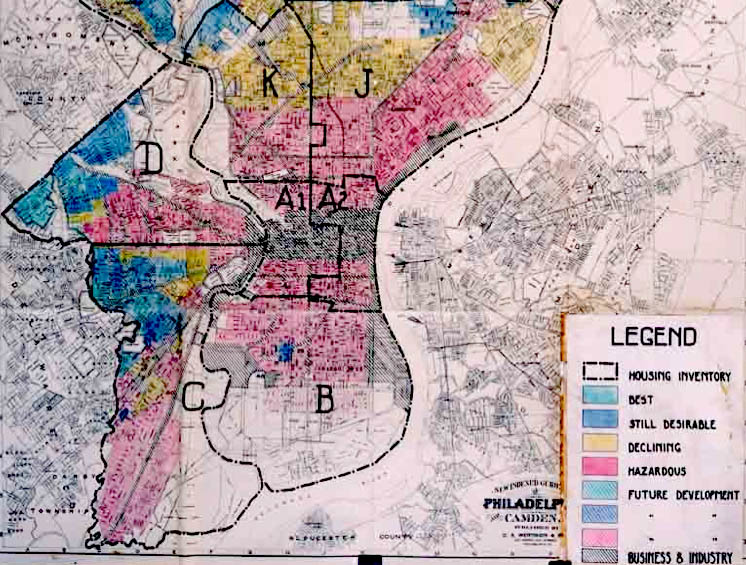
\includegraphics[width=0.8\textwidth]{redliningPhilly.jpg}
        }
                \label{fig:redlining}
    \end{figure}
\end{frame}



\newtheorem{DEFsponsorUSCCR}{Sponsor}
\newtheorem{DEFdataFAIR}{Data}
\begin{frame}
    \frametitle{ Insurance Redlining}
    \begin{DEFsponsorUSCCR} 
        The \href{http://www.usccr.gov/about/}{\textcolor{red}{U.S.~Commission
        on Civil Rights}} examined 
        charges by several Chicago community organizations that insurance 
        companies were redlining their neighborhoods. 
    \end{DEFsponsorUSCCR}
    \vskip.5in
    \begin{DEFdataFAIR}
        The \textcolor{red}{number of FAIR plan policies} written and renewed in Chicago
        by zip code for the number of months of December 1977 through May
        1978.
    \end{DEFdataFAIR}
\end{frame}

\begin{frame}
    \frametitle{ Insurance Redlining}
    Variables to consider:
    \begin{description}
        \item[\texttt{race}] Racial composition in percentage of minority,
        \item[\texttt{fire}] Fire per 100 housing units,
        \item[\texttt{theft}] Theft per 1000 population,
        \item[\texttt{age}] percent of housing unit built before 1939,
        \item[\texttt{involact}] New FAIR plan policies and renewal per 100 housing units,
        \item[\texttt{income}] Median family income in thousands of dollars,
        \item[\texttt{side}] North or South side of Chicago.
    \end{description}
\end{frame}

\newtheorem{DEFecofallacy}{Ecological Fallacy}
\begin{frame}
    \frametitle{Insurance Redlining: Ecological Fallacy}
    \begin{DEFecofallacy}
       When data are collected at the group level, we may observe 
       a correlation between two variables.  The \textcolor{red}{ecological
       fallacy} is concluding that the same correlation holds at the
       individual level. 
    \end{DEFecofallacy}
\end{frame}

\begin{frame}
    \frametitle{Insurance Redlining: Ecological Fallacy}
    \begin{figure}
        \centering
        \caption{1998 annual per capita income and proportion U.S.~born for 50
        states plus D.C.}
        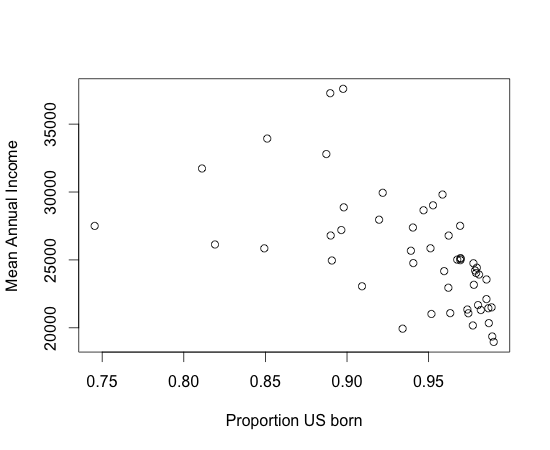
\includegraphics[width=0.75\textwidth]{images/FigureFarawayFigure11dot1.png}
    \end{figure}
\end{frame}

\begin{frame}
    \frametitle{Insurance Redlining: Ecological Fallacy}
    \begin{figure}
        \centering
        \caption{1998 annual per capita income and proportion U.S.~born for 50
        states plus D.C.}
        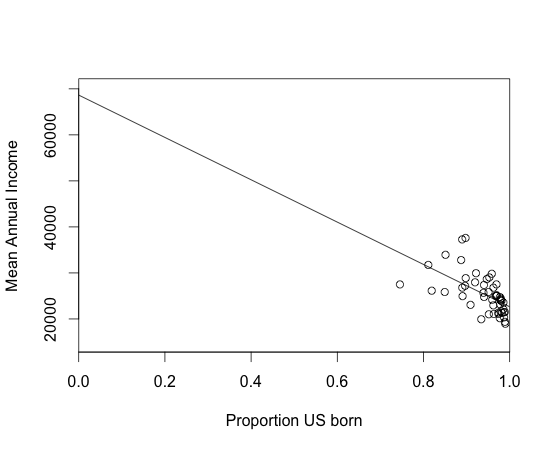
\includegraphics[width=0.75\textwidth]{images/FigureFarawayFigure11dot1b.png}
    \end{figure}
\end{frame}

\begin{frame}[fragile]
    \frametitle{ Insurance Redlining}
    \begin{verse}
For the ecological fallacy example, 
the assumption would be that the incomes of 
the native born do not depend on the proportion of native 
born within the state (and similarly for naturalized citizens).
    \end{verse}
    \vskip0.5in
    \begin{verse}
        For the insurance redlining example, we only have aggregate data.  
        We must inform the sponsor that unless more detailed data becomes
        available, the results for the aggregated data may not hold true 
        at the individual level. 
    \end{verse}
\end{frame}

\begin{frame}[fragile]
    \frametitle{Work Statement: Introduction}
    The work statement should contain a short description 
    of your sponsor.  
    \vskip0.2in
    For the insurance redlining example, 
    \emph{U.S.~Commision on Civil Rights} would be the sponsor.
    \vskip0.2in
    \href{http://en.wikipedia.org/wiki/Boilerplate_%28text%29}{\emph{Boilerplating}} from the sponsor's webpage is often acceptable. 
    \vskip0.5in
    \begin{center}
        \href{http://www.usccr.gov/about/}{http://www.usccr.gov}
    \end{center}
\end{frame}


\begin{frame}   
    \frametitle{Work Statement: Problem Statement}
    \begin{verse}
        Can the insurance companies claim that the discrepancy is due to 
        greater risks in some zip codes?
    \end{verse}
    \vskip0.5in
    \begin{verse}
        The insurance companies could claim that they were denying insurance 
        in neighborhoods where they had sustained large fire-related losses
        and any discriminatory effect was a by-product of legitimate business
        practice.  
    \end{verse}
\end{frame}


\subsection{Sherlock Holmes and the Bicycle Tracks}

\begin{frame}
    \frametitle{Outline}
    \tableofcontents[currentsection, currentsubsection]
\end{frame}

\begin{frame}
    \frametitle{Sherlock Holmes and the Bicycle Tracks: Problem Statement}
    \begin{figure}
        \caption{Which one is the front wheel?}
        \begin{center}
            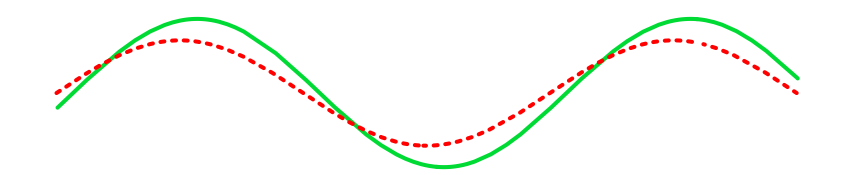
\includegraphics[width=\textwidth]{images/sholmesbike.png}
        \end{center}
        \label{fig:sholmesbike}
    \end{figure}
\end{frame}


\begin{frame}
    \frametitle{Sherlock Holmes and the Bicycle Tracks}
    \begin{verse}
        ``This track, as you perceive, was made by a rider who was going from
        the direction of the school.''
    \end{verse}
    \begin{verse}
        ``Or Toward it?''
    \end{verse}
    \begin{verse}
        ``No, no, my dear Watson.  The more deeply sunk impression is, of
        course, the hind wheel, upon which the weight rests.  You perceive
        several places where it has passed across and obliterated the more
        shallow mark of the front one.  It was undoubtedly heading away from
        the school.''
    \end{verse}
    \hfill -- \textit{The Adventure of the Priory School} by Arthur Conan Doyle
\end{frame}

\begin{frame}
    \frametitle{Sherlock Holmes and the Bicycle Tracks}
    \begin{align*}
        &f_x(t) = r_x(t) +
        \dfrac{L}{\sqrt{1+(r_y^\prime(t)/r_x^\prime(t))^2}}\\
        &f_y(t) = r_y(t) + \dfrac{L r_y^\prime(t)/r_x^\prime(t)}{
        \sqrt{1+ (r_y^\prime(t)/r_x^\prime(t))^2}}
    \end{align*}
\end{frame}

\subsection{Fair Play}
\begin{frame}
    \frametitle{Outline}
    \tableofcontents[currentsection, currentsubsection]
\end{frame}

\begin{frame}
    \frametitle{Is the World Series Fair?: Problem Statement}
    \begin{figure}
        \caption{How can we decide if a game with two competitors is fair?}
            \centering
            \href{http://www.youtube.com/watch?v=WNlCBy07z08}{
            
\includegraphics[width=0.4\textwidth]{Moneyballs.jpg}
            }
    \end{figure}
\end{frame}

\begin{frame}
    \frametitle{Is a Tennis Match Fair?: Problem Statement}
    \begin{figure}
        \caption{How can we decide if a game with two competitors is fair?}
        \begin{center}
            \href{http://www.youtube.com/watch?v=ekQ_Ja02gTY}{
            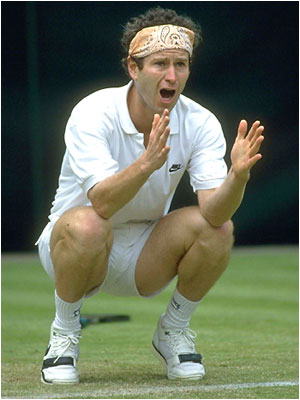
\includegraphics[width=0.4\textwidth]{images/jmcenroe.jpg}}
        \end{center}
        \label{fig:FairGame}
    \end{figure}
\end{frame}


\begin{frame}
    \frametitle{Is a Tennis Match Fair?}
    One simple answer is: 
    \vskip0.2in
    \begin{verse}
        If the roles of the competitors are reversed,
        their probability of winning does not change.
    \end{verse}
    \vskip0.2in
    Isn't that always true?  No.  For example, going first may give a player
    an advantage of disadvantage.
\end{frame}


%\section{Tutorials}

\subsection{\LaTeX}

\begin{frame}
    \frametitle{Programmings in this class}
    \begin{itemize}
        \item \LaTeXs: 
            \begin{itemize}
                \item \texttt{moderncv}
                \item \texttt{beamer}
                \item \texttt{report}
                \item \href{http://www.texample.net}{\texttt{pgf/TikZ}}
            \end{itemize}
        \item Git
            \begin{itemize}
                \item \href{http://git-scm.com/doc}{\texttt{git gui}}
            \end{itemize}
        \item R:
            \begin{itemize}
                \item \texttt{lm}
                \item \href{https://catalyst.library.jhu.edu/catalog/bib_3642743}{\texttt{ggplot2}}
                \item \href{http://www.texample.net/tikz/examples/tikzdevice-demo/}{\texttt{tikzDevice}}
                \item \href{http://www.public.iastate.edu/~dicook/VIGRE/R-packages-slides.pdf}{\texttt{R CMD build}}
            \end{itemize}
    \end{itemize}
\end{frame}


\begin{frame}[fragile]
    \frametitle{Where to get some help for \LaTeXs}
    \begin{center}
    \href{http://en.wikibooks.org/wiki/LaTeX/}{http://en.wikibooks.org/wiki/LaTeX/}
    \end{center}
\end{frame}

\begin{frame}[fragile]
    \frametitle{Tutorial: \LaTeXs}
    \LaTeXs is a computer language for writing a scholarly paper:
    \begin{table}
        \centering
        \caption{HTML vs \LaTeXs}
        \begin{tabular}{c|p{3cm}|p{3cm}}
            \quad   &   HTML    & \LaTeXs \\ 
            \hline
            Code    & 
            \begin{lstlisting}
<html> 
 . . .
</html>
            \end{lstlisting} &  
            \begin{lstlisting}
\begin{document}
 . . .
\end{document}
            \end{lstlisting}\\
            \hline
            Compiler & Firefox and etc. & pdflatex and etc. \\
            \hline
            Output  & Web-page & PDF file
        \end{tabular}
        \label{tab:htmlvslatex}
    \end{table}
\end{frame}

\begin{frame}
    \frametitle{Tutorial: \LaTeXs}
    TeXworks is:
    \begin{itemize}
        \item an editing tool that is separate from \LaTeX,
        \item available in Linux, OSX and Windows,
        \item avaiable in: 
    \end{itemize}
    \vskip0.3in
    \begin{center}
    \href{http://code.google.com/p/texworks/}
    {http://code.google.com/p/texworks/}
    \end{center}
\end{frame}


\begin{frame}[fragile]
    \frametitle{Tutorial: \LaTeXs}
    \begin{itemize}
        \item Demo on preparing a resume using \LaTeXs \texttt{moderncv} package:
            \begin{itemize}
                \item Install \LaTeXs (MikTeX in Windows and MacTeX in OSX),
                \item Download \texttt{moderncv} package files from the course folder,
                \item Change file names to reflect you,
                \item Edit the TeX file,
                \item Compile using your favorite \LaTeXs editor,
                \item Look at the resulting PDF file.
            \end{itemize}
    \end{itemize}
\end{frame}

%\begin{frame}
%    \frametitle{Demo: \LaTeXs}
%    \begin{center}
%        \href{http://cdn.theladders.net/static/pdf/Senator_Obama_Resume.pdf}{In cObama's resume}
%    \end{center}
%\end{frame}

\begin{frame}[fragile]
    \frametitle{Tutorial: \LaTeX}
    Typing mathematics in \LaTeX:
    \begin{lstlisting}
Hello $\int_0^1 \sin(x) dx$ World
\vskip0.5in
Hello $$\int_0^1 \sin(x) dx$$ World
    \end{lstlisting}
    \vskip0.1in
Hello $\int_0^1 \sin(x) dx$ World
\vskip0.5in
Hello $$\int_0^1 \sin(x) dx$$ World
\end{frame}

\begin{frame}[fragile]
    \frametitle{Cautions: \LaTeXs}
    There are numerous quirky \LaTeXs rules:
    \begin{itemize}
        \item opening quotation is not the same as the closing quotation,
        \item period yields \emph{two} blank spaces, 
        \item for \%, need to type \verb+\%+,
        \item for \textbackslash, need to type \verb+\textbackslash+,
        \item for /, need to type /,
        \item for \{, need to type \verb+\{+,
        \item for \$, need to type \verb+\$+,
        \item \verb+~+ yields a single blank space,
        \item and etc.
    \end{itemize}
\end{frame}


\subsection{Git}

\begin{frame}
    \frametitle{The place to get some Git helps}
    \begin{center}
        \href{http://git-scm.com/doc/}{http://git-scm.com/doc/}
    \end{center}
\end{frame}



\newtheorem{POEMbender}{The Blind Men and the Elephant}
\begin{frame}[fragile]
    \frametitle{Demo: \LaTeXs + Git}
    \begin{POEMbender}
        In-class Group Exercise (Scavenger hunt):
    \end{POEMbender}
        \begin{itemize}
            \item Start up a git folder,
            \item Create and edit the \texttt{.gitignore} file,
            \item Download the template for a beamer file,
            \item Look up the poem from the book,
            \item One slide per stanza,
            \item Use \texttt{verse} environment,
            \item Compile after each stanza,
            \item Commit after creating each stanza,
            \item Repeat until done.
        \end{itemize}
\end{frame}

\begin{frame}[fragile]
    \frametitle{Tutorial: Git}

\begin{lstlisting}
sudo apt-get install git
\end{lstlisting}

\begin{figure}[b]
    \caption{An alternative: \texttt{git gui}}
    \begin{center}
        
\includegraphics[height=0.6\textheight]{gitguiinstall.png}
    \end{center}
    \label{fig:gitgui}
\end{figure}
    
\end{frame}

\begin{frame}[fragile]
    \frametitle{Tutorial: Git}

\vspace{8pt}
\begin{lstlisting}
cd ~/
git clone http://cis.jhu.edu/~nhlee/550400.git
\end{lstlisting}

\begin{figure}[b]
    \caption{An alternative: \texttt{git gui}}
    \begin{center}
        
\includegraphics[height=0.5\textheight]{gitgui.png}
    \end{center}
    \label{fig:gitgui2}
\end{figure}
    
\end{frame}

\begin{frame}[fragile]
    \frametitle{Tutorial: Git}
\begin{lstlisting}
cd ~/550400
git reset --hard HEAD
git pull origin master
\end{lstlisting}
\begin{figure}[b]
    \centering
    \caption{An alternative: \texttt{git gui}}
        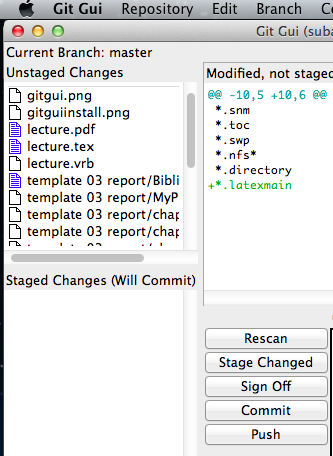
\includegraphics[height=0.6\textheight]{gitguiusing.png}
    \label{fig:gitgui4}
\end{figure}
\end{frame}



\begin{frame}[fragile]
    \frametitle{Tutorial: Git}
    After years of using git, you might find this funny: 
    \begin{columns}
        \begin{column}{0.5\textwidth}
            \begin{figure}
                \begin{center}
                    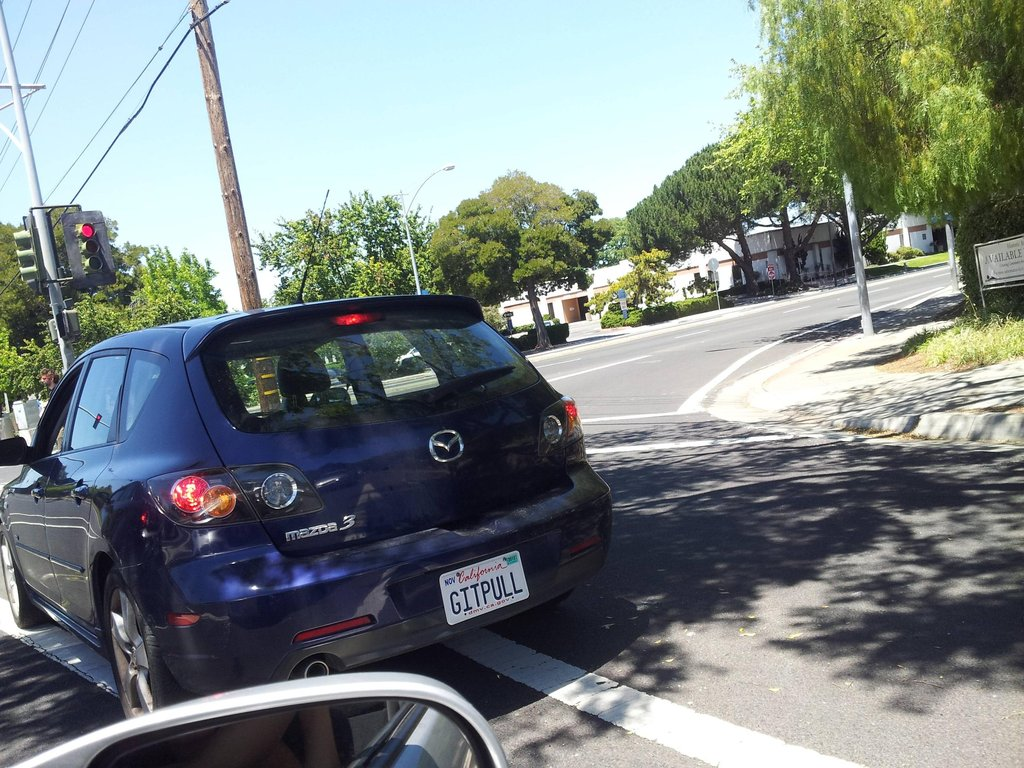
\includegraphics[width=\textwidth]{images/gitpull.jpg}
                \end{center}
            \end{figure}
        \end{column}
        \begin{column}{0.5\textwidth}
            \begin{lstlisting}
git pull origin master
            \end{lstlisting}
        \end{column}
    \end{columns} 
\end{frame}

\begin{frame}[fragile]
    \frametitle{Tutorial: Git}
    After years of using git, you might find this funny: 
    \begin{columns}
        \begin{column}{0.5\textwidth}
            \begin{figure}
                \begin{center}
                    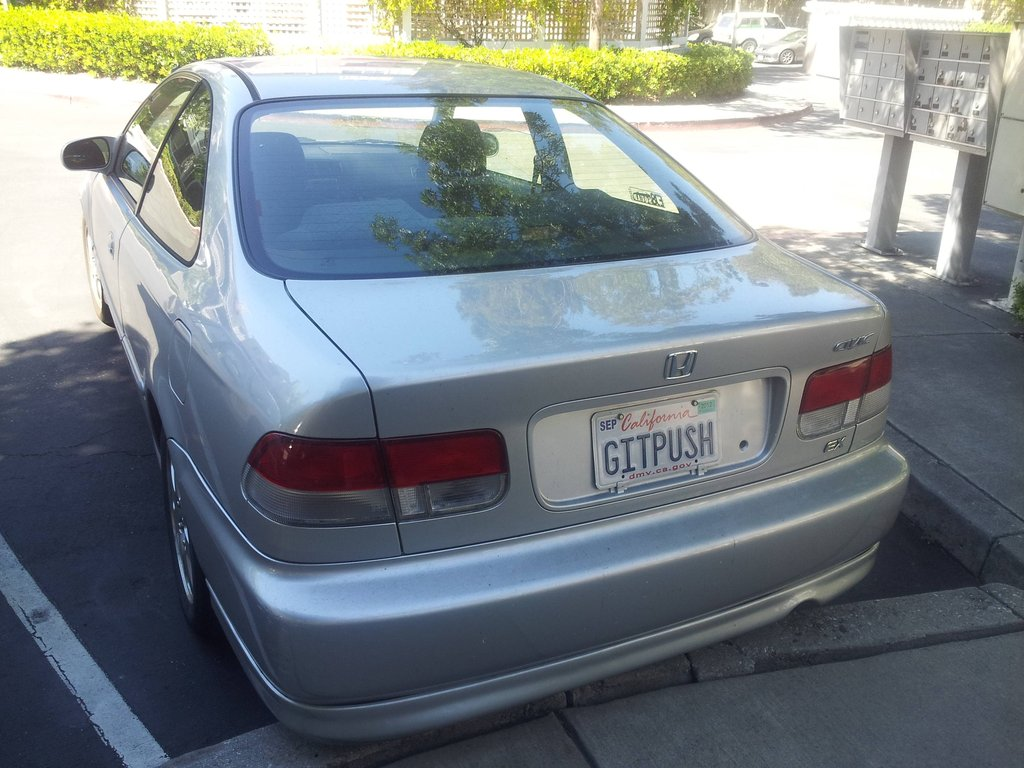
\includegraphics[width=\textwidth]{images/gitpush.jpg}
                \end{center}
            \end{figure}
        \end{column}
        \begin{column}{0.5\textwidth}
            \begin{lstlisting}
git push origin master
            \end{lstlisting}
        \end{column}
    \end{columns} 
\end{frame}

\begin{frame}[fragile]
    \frametitle{Tutorial: Git}
    \begin{columns}
        \begin{column}{0.4\textwidth}
            \begin{figure}
                \caption{For \$19.99, you can also have your own:}
                \begin{center}
                    
\includegraphics[width=\textwidth]{images/gitrdone.jpg}
                \end{center}
            \end{figure}
        \end{column}
        \begin{column}{0.6\textwidth}
\begin{lstlisting}
cd ~/
mkdir hub.git
mkdir computerA.git
mkdir computerB.git

git init --bare hub.git

cd hub.git
cd hooks
cp post-update.sample post-update
\end{lstlisting}
        \end{column}
    \end{columns} 
\end{frame}

\begin{frame}[fragile]
    \frametitle{Tutorial: Git}
    \begin{columns}
        \begin{column}{0.5\textwidth}
\begin{lstlisting}
cd computerA.git
git init 
git remote add origin ~/hub.git
echo 'Hello' >> commonfile.txt
git add commonfile.txt 
git pull origin master
git commit -am 'from A'
git push origin master
\end{lstlisting}
        \end{column}
        \begin{column}{0.5\textwidth}
\begin{lstlisting}
cd computerB.git
git init 
git remote add origin ~/hub.git
echo ' World' >> fileB.txt
git add commonfile.txt 
git pull origin master
git commit -am 'from B'
git push origin master
\end{lstlisting}
        \end{column}
    \end{columns} 
\end{frame}


\begin{frame}[fragile]
    \frametitle{Tutorial: Git}
    \begin{columns}
        \begin{column}{0.5\textwidth}
    \begin{lstlisting}
cd ~/550400

git gui
git reset --hard HEAD

git branch personal
git branch
git checkout personal

edit some file 
git status 
git add . 
git commit -am 'personal edit'

git checkout master
git branch -D personal
    \end{lstlisting}
        \end{column}
        \begin{column}{0.5\textwidth}
    \begin{itemize}
        \item checks if there has been any change to the folder
        \item build and update the \texttt{master} git branch
        \item create and update a \texttt{personal} git branch
    \end{itemize}
        \end{column}
    \end{columns} 
\end{frame}



\begin{frame}
    \frametitle{Tutorial: Git}
    \texttt{.gitignore}?
    \vskip0.1in
    \begin{itemize}
        \item N.B.~the course folder already has one 
        \item Use it to let \emph{git} know the files to \emph{ignore} while
            version controlling
        \item one particular usage: create \texttt{.gitignore} at the root of
            your git folder 
        \item files already been list under the git watch list will not be
            ignored even after creation of \texttt{.gitignore} 
    \end{itemize}
\end{frame}

\subsection{Vim}

\newtheorem{DEFVim}{Vim}
\begin{frame}
    \frametitle{Vim}
    \begin{DEFVim}
        Vim is a \emph{highly customizable} text editor 
    \end{DEFVim}
    \vskip0.1in
    \begin{enumerate}
        \item \LaTeX, R, C/C++, Java, Python, Git and etc.
        \item Regular expression, syntax coloring, autocompletion
        \item Try Firefox + Wasavi/Vimperator/Vimium
        \item \texttt{<ESC>}-mode
        \begin{itemize}
            \item \texttt{:}-mode, aka., the last line mode
            \item \texttt{i}-mode, aka., the insert mode
        \end{itemize}
    \end{enumerate}
\end{frame}

\subsection{R}

\begin{frame}[fragile]
    \frametitle{Demo: R + \LaTeX}
    \begin{columns}
        \begin{column}{0.5\textwidth}
            \begin{figure}
                \centering
            \caption{R Studio}
            \href{http://rstudio.org}{
            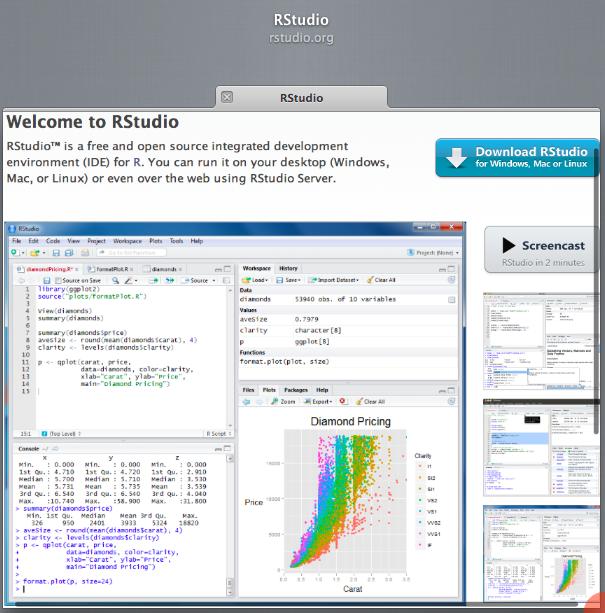
\includegraphics[width=\textwidth]{images/Rstudio}
            }
        \end{figure}
        \end{column}
        \begin{column}{0.5\textwidth}
            \begin{figure}
                \centering
                        \caption{R}
                    \href{http://www.r-project.org}{
                        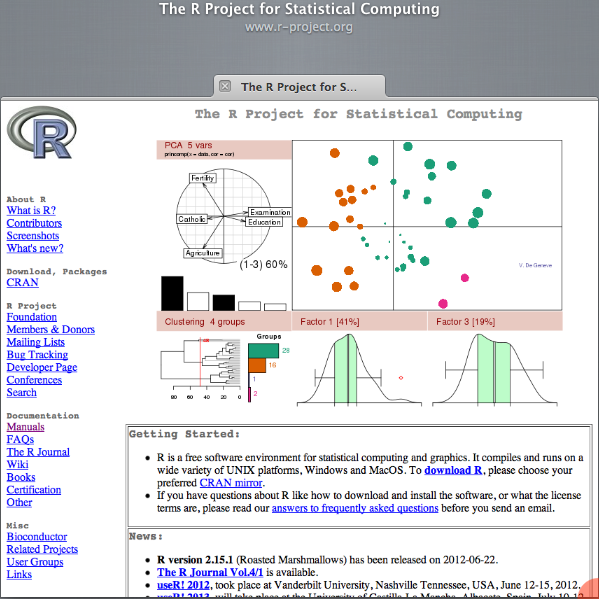
\includegraphics[width=\textwidth]{images/Rproject}}
            \end{figure}
        \end{column}
    \end{columns} 
\end{frame}

\begin{frame}[fragile]
    \frametitle{Demo: R + \LaTeX}
    \begin{columns}
        \begin{column}{0.45\textwidth}
    \begin{lstlisting}
install.packages(faraway)
install.packages(tikzDevice)
require(faraway)
require(tikzDevice)
data(eco)
tikz('embeddedfig1.tex', 
    standAlone=F, 
    width=5,height=5)
plot(income ~ usborn, 
    data=eco,
    xlab=`Proportion US born'
    ylab=`Mean Annual Income'
    )
dev.off()
    \end{lstlisting}
        \end{column}
        \begin{column}{0.55\textwidth}
        \begin{figure}[0.8\textwidth]
            % Created by tikzDevice version 0.6.2 on 2012-09-11 12:28:03
% !TEX encoding = UTF-8 Unicode
\begin{tikzpicture}[x=1pt,y=1pt,scale=0.5]
\definecolor[named]{drawColor}{rgb}{0.00,0.00,0.00}
\definecolor[named]{fillColor}{rgb}{1.00,1.00,1.00}
\fill[color=fillColor,fill opacity=0.00,] (0,0) rectangle (361.35,361.35);
\begin{scope}
\path[clip] ( 49.20, 61.20) rectangle (336.15,312.15);
\definecolor[named]{fillColor}{rgb}{0.00,0.00,0.00}
\definecolor[named]{drawColor}{rgb}{0.00,0.00,0.00}

\draw[color=drawColor,line cap=round,line join=round,fill opacity=0.00,] (321.92,101.46) circle (  2.25);

\draw[color=drawColor,line cap=round,line join=round,fill opacity=0.00,] (270.39,154.23) circle (  2.25);

\draw[color=drawColor,line cap=round,line join=round,fill opacity=0.00,] (237.82,121.63) circle (  2.25);

\draw[color=drawColor,line cap=round,line join=round,fill opacity=0.00,] (322.27, 87.80) circle (  2.25);

\draw[color=drawColor,line cap=round,line join=round,fill opacity=0.00,] ( 59.83,177.01) circle (  2.25);

\draw[color=drawColor,line cap=round,line join=round,fill opacity=0.00,] (278.80,191.40) circle (  2.25);

\draw[color=drawColor,line cap=round,line join=round,fill opacity=0.00,] (225.25,302.86) circle (  2.25);

\draw[color=drawColor,line cap=round,line join=round,fill opacity=0.00,] (291.43,205.82) circle (  2.25);

\draw[color=drawColor,line cap=round,line join=round,fill opacity=0.00,] (216.67,298.87) circle (  2.25);

\draw[color=drawColor,line cap=round,line join=round,fill opacity=0.00,] (172.76,156.43) circle (  2.25);

\draw[color=drawColor,line cap=round,line join=round,fill opacity=0.00,] (301.22,146.06) circle (  2.25);

\draw[color=drawColor,line cap=round,line join=round,fill opacity=0.00,] (139.93,159.99) circle (  2.25);

\draw[color=drawColor,line cap=round,line join=round,fill opacity=0.00,] (296.56, 96.96) circle (  2.25);

\draw[color=drawColor,line cap=round,line join=round,fill opacity=0.00,] (225.68,194.09) circle (  2.25);

\draw[color=drawColor,line cap=round,line join=round,fill opacity=0.00,] (313.14,136.08) circle (  2.25);

\draw[color=drawColor,line cap=round,line join=round,fill opacity=0.00,] (315.76,132.41) circle (  2.25);

\draw[color=drawColor,line cap=round,line join=round,fill opacity=0.00,] (303.32,145.58) circle (  2.25);

\draw[color=drawColor,line cap=round,line join=round,fill opacity=0.00,] (324.10,102.26) circle (  2.25);

\draw[color=drawColor,line cap=round,line join=round,fill opacity=0.00,] (307.96,100.26) circle (  2.25);

\draw[color=drawColor,line cap=round,line join=round,fill opacity=0.00,] (295.32,120.28) circle (  2.25);

\draw[color=drawColor,line cap=round,line join=round,fill opacity=0.00,] (251.62,207.43) circle (  2.25);

\draw[color=drawColor,line cap=round,line join=round,fill opacity=0.00,] (214.06,243.01) circle (  2.25);

\draw[color=drawColor,line cap=round,line join=round,fill opacity=0.00,] (283.42,156.50) circle (  2.25);

\draw[color=drawColor,line cap=round,line join=round,fill opacity=0.00,] (303.14,177.10) circle (  2.25);

\draw[color=drawColor,line cap=round,line join=round,fill opacity=0.00,] (325.52, 70.49) circle (  2.25);

\draw[color=drawColor,line cap=round,line join=round,fill opacity=0.00,] (314.27,138.67) circle (  2.25);

\draw[color=drawColor,line cap=round,line join=round,fill opacity=0.00,] (311.62, 85.63) circle (  2.25);

\draw[color=drawColor,line cap=round,line join=round,fill opacity=0.00,] (312.00,142.75) circle (  2.25);

\draw[color=drawColor,line cap=round,line join=round,fill opacity=0.00,] (224.04,173.24) circle (  2.25);

\draw[color=drawColor,line cap=round,line join=round,fill opacity=0.00,] (285.10,195.95) circle (  2.25);

\draw[color=drawColor,line cap=round,line join=round,fill opacity=0.00,] (174.71,257.22) circle (  2.25);

\draw[color=drawColor,line cap=round,line join=round,fill opacity=0.00,] (264.86, 82.69) circle (  2.25);

\draw[color=drawColor,line cap=round,line join=round,fill opacity=0.00,] (131.29,229.76) circle (  2.25);

\draw[color=drawColor,line cap=round,line join=round,fill opacity=0.00,] (313.79,133.80) circle (  2.25);

\draw[color=drawColor,line cap=round,line join=round,fill opacity=0.00,] (315.08,104.36) circle (  2.25);

\draw[color=drawColor,line cap=round,line join=round,fill opacity=0.00,] (303.42,147.48) circle (  2.25);

\draw[color=drawColor,line cap=round,line join=round,fill opacity=0.00,] (308.62, 96.85) circle (  2.25);

\draw[color=drawColor,line cap=round,line join=round,fill opacity=0.00,] (271.97,142.90) circle (  2.25);

\draw[color=drawColor,line cap=round,line join=round,fill opacity=0.00,] (295.52,168.15) circle (  2.25);

\draw[color=drawColor,line cap=round,line join=round,fill opacity=0.00,] (216.98,168.21) circle (  2.25);

\draw[color=drawColor,line cap=round,line join=round,fill opacity=0.00,] (316.94, 99.80) circle (  2.25);

\draw[color=drawColor,line cap=round,line join=round,fill opacity=0.00,] (320.67,109.84) circle (  2.25);

\draw[color=drawColor,line cap=round,line join=round,fill opacity=0.00,] (320.71,127.85) circle (  2.25);

\draw[color=drawColor,line cap=round,line join=round,fill opacity=0.00,] (217.76,145.28) circle (  2.25);

\draw[color=drawColor,line cap=round,line join=round,fill opacity=0.00,] (284.06, 96.19) circle (  2.25);

\draw[color=drawColor,line cap=round,line join=round,fill opacity=0.00,] (292.53,135.53) circle (  2.25);

\draw[color=drawColor,line cap=round,line join=round,fill opacity=0.00,] (271.72,175.54) circle (  2.25);

\draw[color=drawColor,line cap=round,line join=round,fill opacity=0.00,] (249.19,182.72) circle (  2.25);

\draw[color=drawColor,line cap=round,line join=round,fill opacity=0.00,] (324.52, 75.53) circle (  2.25);

\draw[color=drawColor,line cap=round,line join=round,fill opacity=0.00,] (303.47,146.80) circle (  2.25);

\draw[color=drawColor,line cap=round,line join=round,fill opacity=0.00,] (312.30,122.96) circle (  2.25);
\end{scope}
\begin{scope}
\path[clip] (  0.00,  0.00) rectangle (361.35,361.35);
\definecolor[named]{fillColor}{rgb}{0.00,0.00,0.00}
\definecolor[named]{drawColor}{rgb}{0.00,0.00,0.00}

\draw[color=drawColor,line cap=round,line join=round,fill opacity=0.00,] ( 64.82, 61.20) -- (282.19, 61.20);

\draw[color=drawColor,line cap=round,line join=round,fill opacity=0.00,] ( 64.82, 61.20) -- ( 64.82, 55.20);

\draw[color=drawColor,line cap=round,line join=round,fill opacity=0.00,] (119.16, 61.20) -- (119.16, 55.20);

\draw[color=drawColor,line cap=round,line join=round,fill opacity=0.00,] (173.50, 61.20) -- (173.50, 55.20);

\draw[color=drawColor,line cap=round,line join=round,fill opacity=0.00,] (227.85, 61.20) -- (227.85, 55.20);

\draw[color=drawColor,line cap=round,line join=round,fill opacity=0.00,] (282.19, 61.20) -- (282.19, 55.20);

\node[color=drawColor,anchor=base,inner sep=0pt, outer sep=0pt, scale=  1.00] at ( 64.82, 37.20) {\tiny 0.75};
\node[color=drawColor,anchor=base,inner sep=0pt, outer sep=0pt, scale=  1.00] at (119.16, 37.20) {\tiny 0.80};
\node[color=drawColor,anchor=base,inner sep=0pt, outer sep=0pt, scale=  1.00] at (173.50, 37.20) {\tiny 0.85};
\node[color=drawColor,anchor=base,inner sep=0pt, outer sep=0pt, scale=  1.00] at (227.85, 37.20) {\tiny 0.90};
\node[color=drawColor,anchor=base,inner sep=0pt, outer sep=0pt, scale=  1.00] at (282.19, 37.20) {\tiny 0.95};

\draw[color=drawColor,line cap=round,line join=round,fill opacity=0.00,] ( 49.20, 83.48) -- ( 49.20,270.47);

\draw[color=drawColor,line cap=round,line join=round,fill opacity=0.00,] ( 49.20, 83.48) -- ( 43.20, 83.48);

\draw[color=drawColor,line cap=round,line join=round,fill opacity=0.00,] ( 49.20,145.81) -- ( 43.20,145.81);

\draw[color=drawColor,line cap=round,line join=round,fill opacity=0.00,] ( 49.20,208.14) -- ( 43.20,208.14);

\draw[color=drawColor,line cap=round,line join=round,fill opacity=0.00,] ( 49.20,270.47) -- ( 43.20,270.47);

\node[rotate= 90.00,color=drawColor,anchor=base,inner sep=0pt, outer sep=0pt,
scale=  1.00] at ( 37.20, 83.48) {\tiny 20000};

\node[rotate= 90.00,color=drawColor,anchor=base,inner sep=0pt, outer sep=0pt,
scale=  1.00] at ( 37.20,145.81) {\tiny 25000};

\node[rotate= 90.00,color=drawColor,anchor=base,inner sep=0pt, outer sep=0pt,
scale=  1.00] at ( 37.20,208.14) {\tiny 30000};

\node[rotate= 90.00,color=drawColor,anchor=base,inner sep=0pt, outer sep=0pt,
scale=  1.00] at ( 37.20,270.47) {\tiny 35000};

\draw[color=drawColor,line cap=round,line join=round,fill opacity=0.00,] ( 49.20, 61.20) --
	(336.15, 61.20) --
	(336.15,312.15) --
	( 49.20,312.15) --
	( 49.20, 61.20);
\end{scope}
\begin{scope}
\path[clip] (  0.00,  0.00) rectangle (361.35,361.35);
\definecolor[named]{fillColor}{rgb}{0.00,0.00,0.00}
\definecolor[named]{drawColor}{rgb}{0.00,0.00,0.00}

\node[color=drawColor,anchor=base,inner sep=0pt, outer sep=0pt, scale=  1.00]
at (192.67, 13.20) {USborn};

\node[rotate= 90.00,color=drawColor,anchor=base,inner sep=0pt, outer sep=0pt,
scale=  1.00] at ( 13.20,186.67) {Income};
\end{scope}
\end{tikzpicture}

        \end{figure}
        \end{column}
    \end{columns} 
\end{frame}

\begin{frame}[fragile]
    \frametitle{Demo: R + \LaTeX}
    \begin{columns}
        \begin{column}{0.45\textwidth}
            \begin{lstlisting}
tikz('embeddedfig2.tex', 
    standAlone=F, 
    width=5,height=5)
plot(income ~ usborn, 
    data = eco,
    xlab=`Proportion US born',
    ylab=`Mean Annual Income',
    xlim=c(0,1),
    ylim=c(15000,70000),
    xaxs='i')
g<-lm(income~usborn,eco)
abline(coef(g))
dev.off()
            \end{lstlisting}
        \end{column}
        \begin{column}{0.55\textwidth}
            % Created by tikzDevice version 0.6.2 on 2012-09-11 13:10:12
% !TEX encoding = UTF-8 Unicode
\begin{tikzpicture}[x=1pt,y=1pt,scale=0.5]
\definecolor[named]{drawColor}{rgb}{0.00,0.00,0.00}
\definecolor[named]{fillColor}{rgb}{1.00,1.00,1.00}
\fill[color=fillColor,fill opacity=0.00,] (0,0) rectangle (361.35,361.35);
\begin{scope}
\path[clip] ( 49.20, 61.20) rectangle (336.15,312.15);
\definecolor[named]{drawColor}{rgb}{0.00,0.00,0.00}

\draw[color=drawColor,line cap=round,line join=round,fill opacity=0.00,] (332.29, 97.71) circle (  2.25);

\draw[color=drawColor,line cap=round,line join=round,fill opacity=0.00,] (318.69,115.59) circle (  2.25);

\draw[color=drawColor,line cap=round,line join=round,fill opacity=0.00,] (310.09,104.55) circle (  2.25);

\draw[color=drawColor,line cap=round,line join=round,fill opacity=0.00,] (332.39, 93.08) circle (  2.25);

\draw[color=drawColor,line cap=round,line join=round,fill opacity=0.00,] (263.10,123.32) circle (  2.25);

\draw[color=drawColor,line cap=round,line join=round,fill opacity=0.00,] (320.91,128.19) circle (  2.25);

\draw[color=drawColor,line cap=round,line join=round,fill opacity=0.00,] (306.77,165.97) circle (  2.25);

\draw[color=drawColor,line cap=round,line join=round,fill opacity=0.00,] (324.24,133.08) circle (  2.25);

\draw[color=drawColor,line cap=round,line join=round,fill opacity=0.00,] (304.51,164.61) circle (  2.25);

\draw[color=drawColor,line cap=round,line join=round,fill opacity=0.00,] (292.91,116.34) circle (  2.25);

\draw[color=drawColor,line cap=round,line join=round,fill opacity=0.00,] (326.83,112.83) circle (  2.25);

\draw[color=drawColor,line cap=round,line join=round,fill opacity=0.00,] (284.24,117.55) circle (  2.25);

\draw[color=drawColor,line cap=round,line join=round,fill opacity=0.00,] (325.60, 96.19) circle (  2.25);

\draw[color=drawColor,line cap=round,line join=round,fill opacity=0.00,] (306.88,129.10) circle (  2.25);

\draw[color=drawColor,line cap=round,line join=round,fill opacity=0.00,] (329.97,109.44) circle (  2.25);

\draw[color=drawColor,line cap=round,line join=round,fill opacity=0.00,] (330.67,108.20) circle (  2.25);

\draw[color=drawColor,line cap=round,line join=round,fill opacity=0.00,] (327.38,112.66) circle (  2.25);

\draw[color=drawColor,line cap=round,line join=round,fill opacity=0.00,] (332.87, 97.98) circle (  2.25);

\draw[color=drawColor,line cap=round,line join=round,fill opacity=0.00,] (328.61, 97.30) circle (  2.25);

\draw[color=drawColor,line cap=round,line join=round,fill opacity=0.00,] (325.27,104.09) circle (  2.25);

\draw[color=drawColor,line cap=round,line join=round,fill opacity=0.00,] (313.73,133.62) circle (  2.25);

\draw[color=drawColor,line cap=round,line join=round,fill opacity=0.00,] (303.82,145.68) circle (  2.25);

\draw[color=drawColor,line cap=round,line join=round,fill opacity=0.00,] (322.13,116.36) circle (  2.25);

\draw[color=drawColor,line cap=round,line join=round,fill opacity=0.00,] (327.33,123.35) circle (  2.25);

\draw[color=drawColor,line cap=round,line join=round,fill opacity=0.00,] (333.24, 87.22) circle (  2.25);

\draw[color=drawColor,line cap=round,line join=round,fill opacity=0.00,] (330.27,110.32) circle (  2.25);

\draw[color=drawColor,line cap=round,line join=round,fill opacity=0.00,] (329.57, 92.34) circle (  2.25);

\draw[color=drawColor,line cap=round,line join=round,fill opacity=0.00,] (329.67,111.70) circle (  2.25);

\draw[color=drawColor,line cap=round,line join=round,fill opacity=0.00,] (306.45,122.04) circle (  2.25);

\draw[color=drawColor,line cap=round,line join=round,fill opacity=0.00,] (322.57,129.73) circle (  2.25);

\draw[color=drawColor,line cap=round,line join=round,fill opacity=0.00,] (293.43,150.50) circle (  2.25);

\draw[color=drawColor,line cap=round,line join=round,fill opacity=0.00,] (317.23, 91.35) circle (  2.25);

\draw[color=drawColor,line cap=round,line join=round,fill opacity=0.00,] (281.96,141.19) circle (  2.25);

\draw[color=drawColor,line cap=round,line join=round,fill opacity=0.00,] (330.15,108.67) circle (  2.25);

\draw[color=drawColor,line cap=round,line join=round,fill opacity=0.00,] (330.49, 98.69) circle (  2.25);

\draw[color=drawColor,line cap=round,line join=round,fill opacity=0.00,] (327.41,113.31) circle (  2.25);

\draw[color=drawColor,line cap=round,line join=round,fill opacity=0.00,] (328.78, 96.15) circle (  2.25);

\draw[color=drawColor,line cap=round,line join=round,fill opacity=0.00,] (319.11,111.75) circle (  2.25);

\draw[color=drawColor,line cap=round,line join=round,fill opacity=0.00,] (325.32,120.31) circle (  2.25);

\draw[color=drawColor,line cap=round,line join=round,fill opacity=0.00,] (304.59,120.33) circle (  2.25);

\draw[color=drawColor,line cap=round,line join=round,fill opacity=0.00,] (330.98, 97.15) circle (  2.25);

\draw[color=drawColor,line cap=round,line join=round,fill opacity=0.00,] (331.96,100.55) circle (  2.25);

\draw[color=drawColor,line cap=round,line join=round,fill opacity=0.00,] (331.97,106.65) circle (  2.25);

\draw[color=drawColor,line cap=round,line join=round,fill opacity=0.00,] (304.79,112.56) circle (  2.25);

\draw[color=drawColor,line cap=round,line join=round,fill opacity=0.00,] (322.30, 95.92) circle (  2.25);

\draw[color=drawColor,line cap=round,line join=round,fill opacity=0.00,] (324.53,109.26) circle (  2.25);

\draw[color=drawColor,line cap=round,line join=round,fill opacity=0.00,] (319.04,122.82) circle (  2.25);

\draw[color=drawColor,line cap=round,line join=round,fill opacity=0.00,] (313.09,125.25) circle (  2.25);

\draw[color=drawColor,line cap=round,line join=round,fill opacity=0.00,] (332.98, 88.92) circle (  2.25);

\draw[color=drawColor,line cap=round,line join=round,fill opacity=0.00,] (327.42,113.08) circle (  2.25);

\draw[color=drawColor,line cap=round,line join=round,fill opacity=0.00,] (329.75,105.00) circle (  2.25);
\end{scope}
\begin{scope}
\path[clip] (  0.00,  0.00) rectangle (361.35,361.35);
\definecolor[named]{drawColor}{rgb}{0.00,0.00,0.00}

\draw[color=drawColor,line cap=round,line join=round,fill opacity=0.00,] ( 49.20, 61.20) -- (336.15, 61.20);

\draw[color=drawColor,line cap=round,line join=round,fill opacity=0.00,] ( 49.20, 61.20) -- ( 49.20, 55.20);

\draw[color=drawColor,line cap=round,line join=round,fill opacity=0.00,] (106.59, 61.20) -- (106.59, 55.20);

\draw[color=drawColor,line cap=round,line join=round,fill opacity=0.00,] (163.98, 61.20) -- (163.98, 55.20);

\draw[color=drawColor,line cap=round,line join=round,fill opacity=0.00,] (221.37, 61.20) -- (221.37, 55.20);

\draw[color=drawColor,line cap=round,line join=round,fill opacity=0.00,] (278.76, 61.20) -- (278.76, 55.20);

\draw[color=drawColor,line cap=round,line join=round,fill opacity=0.00,] (336.15, 61.20) -- (336.15, 55.20);

\node[color=drawColor,anchor=base,inner sep=0pt, outer sep=0pt, scale=  1.00]
at ( 49.20, 37.20) {\tiny 0.0};

\node[color=drawColor,anchor=base,inner sep=0pt, outer sep=0pt, scale=  1.00] at (106.59, 37.20) {\tiny 0.2};

\node[color=drawColor,anchor=base,inner sep=0pt, outer sep=0pt, scale=  1.00] at (163.98, 37.20) {\tiny 0.4};

\node[color=drawColor,anchor=base,inner sep=0pt, outer sep=0pt, scale=  1.00] at (221.37, 37.20) {\tiny 0.6};

\node[color=drawColor,anchor=base,inner sep=0pt, outer sep=0pt, scale=  1.00] at (278.76, 37.20) {\tiny 0.8};

\node[color=drawColor,anchor=base,inner sep=0pt, outer sep=0pt, scale=  1.00] at (336.15, 37.20) {\tiny 1.0};

\draw[color=drawColor,line cap=round,line join=round,fill opacity=0.00,] ( 49.20, 91.62) -- ( 49.20,302.86);

\draw[color=drawColor,line cap=round,line join=round,fill opacity=0.00,] ( 49.20, 91.62) -- ( 43.20, 91.62);

\draw[color=drawColor,line cap=round,line join=round,fill opacity=0.00,] ( 49.20,133.87) -- ( 43.20,133.87);

\draw[color=drawColor,line cap=round,line join=round,fill opacity=0.00,] ( 49.20,176.11) -- ( 43.20,176.11);

\draw[color=drawColor,line cap=round,line join=round,fill opacity=0.00,] ( 49.20,218.36) -- ( 43.20,218.36);

\draw[color=drawColor,line cap=round,line join=round,fill opacity=0.00,] ( 49.20,260.61) -- ( 43.20,260.61);

\draw[color=drawColor,line cap=round,line join=round,fill opacity=0.00,] ( 49.20,302.86) -- ( 43.20,302.86);

\node[rotate= 90.00,color=drawColor,anchor=base,inner sep=0pt, outer sep=0pt,
scale=  1.00] at ( 37.20, 91.62) {\tiny 20000};

\node[rotate= 90.00,color=drawColor,anchor=base,inner sep=0pt, outer sep=0pt, scale=  1.00] at ( 37.20,133.87) {\tiny 30000};
\node[rotate= 90.00,color=drawColor,anchor=base,inner sep=0pt, outer sep=0pt, scale=  1.00] at ( 37.20,176.11) {\tiny 40000};
\node[rotate= 90.00,color=drawColor,anchor=base,inner sep=0pt, outer sep=0pt, scale=  1.00] at ( 37.20,218.36) {\tiny 50000};
\node[rotate= 90.00,color=drawColor,anchor=base,inner sep=0pt, outer sep=0pt, scale=  1.00] at ( 37.20,260.61) {\tiny 60000};
\node[rotate= 90.00,color=drawColor,anchor=base,inner sep=0pt, outer sep=0pt, scale=  1.00] at ( 37.20,302.86) {\tiny 70000};

\draw[color=drawColor,line cap=round,line join=round,fill opacity=0.00,] 
    ( 49.20, 61.20) --
	(336.15, 61.20) --
	(336.15,312.15) --
	( 49.20,312.15) --
	( 49.20, 61.20);
\end{scope}
\begin{scope}
\path[clip] (  0.00,  0.00) rectangle (361.35,361.35);
\definecolor[named]{drawColor}{rgb}{0.00,0.00,0.00}

\node[color=drawColor,anchor=base,inner sep=0pt, outer sep=0pt, scale=  1.00] at (192.68, 13.20) {Proportion US born};

\node[rotate= 90.00,color=drawColor,anchor=base,inner sep=0pt, outer sep=0pt, scale=  1.00] at ( 13.20,186.67) {Mean Annual Income};
\end{scope}
\begin{scope}
\path[clip] ( 49.20, 61.20) rectangle (336.15,312.15);
\definecolor[named]{drawColor}{rgb}{0.00,0.00,0.00}

\draw[color=drawColor,line cap=round,line join=round,fill opacity=0.00,] ( 49.20,297.12) -- (336.15,102.70);
\end{scope}
\end{tikzpicture}

        \end{column}
    \end{columns} 
\end{frame}

%\section{Exercises}

\begin{frame}[allowframebreaks]
    \frametitle{Outline}
    \tableofcontents[currentsection, currentsubsection]
\end{frame}

\begin{frame}
    \frametitle{WMA Problem 2.5a \& 2.6a}
        \begin{verse}
            The Williams family's income of \$25,000 falls below 185\% of the 
            \href{http://aspe.hhs.gov/poverty/12poverty.shtml}{Federal Poverty
            Threshold} for a family of four, qualifying them
            for food stamps. 
        \end{verse}
        \vskip0.3in
\begin{description}
    \item[Problem 2.5a] {Identify terms that need to be defined or restated
        for a nontechnical audience}
    \item[Problem 2.6a] Rewrite the sentences in the previous questions for an
        audience with a fifth-grade education.  Convey the main point,
        not the calculation or the jargon. 
    \item[FYI] \href{http://www.bloomberg.com/video/how-the-rich-get-richer-and-the-poor-poorer-kfuILNN9SoaQXLd5cVBwPQ.html}{Off-the-chart}
\end{description}
\end{frame}

\begin{frame}
    \frametitle{WMA Problem 2.8a}
    Rewrite each of these sentences to specify the direction and magnitude of
    the association:
    \vskip0.1in
    \begin{center}
    \begin{verse}
        In the United States, race is correlated with income. 
    \end{verse}
    \end{center}
    \begin{table}
        \centering
        \caption{\textbf{Median income by race and Hispanic origin, United States, 1999}}
        \label{tab:WMAex2x8}
        \begin{tabular}{lc}
        Race/Hispanic origin & Median Income \\
        \hline 
        White   & \$42,504 \\
        Black   & \$27,910 \\ 
        Asian/Pacific Islander   & \$51,205 \\ 
        Hispanic (can be of any race) & \$30,735 \\
        \hline
        \end{tabular}
    \end{table}
\end{frame}

\begin{frame}
    \frametitle{WMA Problem 2.9}
    Use the GEE approach to describe the patterns in the figure below,
    including an introductory sentence about the purpose of the chart 
    before summarizing the patterns. 
    \begin{figure}
        \begin{center}
            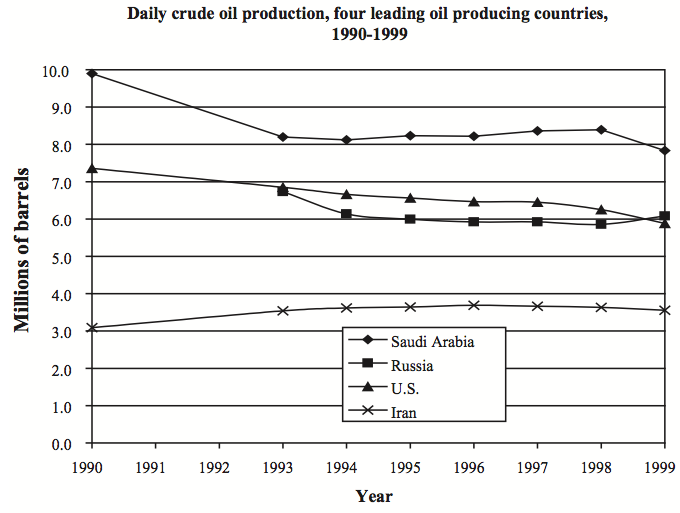
\includegraphics[width=0.6\textwidth]{images/WMAex2x9.png}
        \end{center}
    \end{figure}
\end{frame}

\begin{frame}
    \frametitle{IMM Problem 1.1}
    Suppose people enter the elevators in a skyscraper at random during the
    morning rush. The result will be several elevators stopping on each floor
    to discharge one or two passengers each. 
    \vskip0.1in
    \begin{itemize}
        \item Discuss schemes for improving the situation. 
        \item How could improvement be measured? 
        \item How could you model the situation to decide what scheme to adopt?
    \end{itemize}
\end{frame}

\begin{frame}
    \frametitle{IMM Problem 1.6}
    Unless you have been extremely lucky, you have had a large class in a
    poorly designed lecture hall. 
    
    \vskip0.25in
    \begin{description}
        \item[(a)] What are some criteria to be considered
    in designing a large lecture hall? 
    \end{description}
\end{frame}
    
\begin{frame}
    \frametitle{IMM Problem 1.6}
    Unless you have been extremely lucky, you have had a large class in a
    poorly designed lecture hall. 
    \vskip0.15in
    \begin{description}
        \item[(b)] One criterion is legibility of material written on the boards. 
        \begin{itemize}
            \item Construct a model of legibility as a function of 
                \begin{itemize}
                    \item  \emph{the distance} your seat is from the board 
                    \item \emph{the angle} at which you look at the board 
                \end{itemize}
            \item What will the curves of constant legibility look like on a
                floor plan?
            \item How can you test this prediction? Try it. 
            \item Does this suggest shaping the back of the hall differently
                than is usually done? How?
        \end{itemize}    
    \end{description}
    \vfill
\end{frame}
     
\begin{frame}
    \frametitle{IMM Problem 1.6}
    Unless you have been extremely lucky, you have had a large class in a
    poorly designed lecture hall. 
    
    \vskip0.25in
    \begin{description}
        \item[(c)] Can mathematical modeling help with any other criteria
    besides the one mentioned in (b)? Try to pick a criterion from among these
    possibilities and develop a model for it.
    \end{description}
\end{frame}



\newtheorem{POEMbender}{The Blind Men and the Elephant}
\begin{frame}[fragile]
    \frametitle{Collect All: \LaTeXs + Git}
    \begin{POEMbender}
        In-class Group Exercise (Scavenger hunt):
    \end{POEMbender}
        \begin{itemize}
            \item Start up a git folder,
            \item Create and edit the \texttt{.gitignore} file,
            \item Download the template for a beamer file,
            \item Look up the poem from the book,
            \item One slide per stanza,
            \item Use \texttt{verse} environment,
            \item Compile after each stanza,
            \item Commit after creating each stanza,
            \item Repeat until done.
        \end{itemize}
\end{frame}

%\section{Project}

\begin{frame}
    \frametitle{Outline}
    \tableofcontents[currentsection, currentsubsection]
\end{frame}


\begin{frame}[fragile]
    \frametitle{Mission Impossible?: an analogy}
    \begin{figure}
        \caption{Mission Impossible Season 2 Episode (00:00 -- 06:25)}
    \begin{center}
    \href{http://movies.netflix.com/WiPlayer?movieid=70157337&trkid=4431095&pt_request_id=a8a7108c-c068-4d22-b649-0b7095279045-1882594&pt_rank=4&pt_row=-1&pt_location=WATCHNOW#MovieId=70157337&EpisodeMovieId=70156671}{
            
\includegraphics[width=0.8\textwidth]{images/IMFproblemstatement.png}
    }
    \end{center}
    \end{figure}
\end{frame}

\begin{frame}
    \frametitle{Project in Industry: Frequently Recurring Elements}
    A stylized timeline:
    \vspace{7pt}
             \begin{enumerate}
                 \item Work Statement,
                 \item Midterm Presentation,
                 \item Progress Report,
                 \item Final Presentation,
                 \item Final Report.
             \end{enumerate}
    \begin{center}
        \href{http://www.ipam.ucla.edu/programs/rips2011/}{
        
\includegraphics[width=0.5\textwidth]{images/ipam}}        
    \end{center}
\end{frame}

\subsection{Work Statement}

\begin{frame}
    \frametitle{Outline}
    \tableofcontents[currentsection, currentsubsection]
\end{frame}

\begin{frame}
    \frametitle{What is Work Statement}
This is the written proposal and definition of the project and constitutes the
team's ``contract'' with the sponsor. It should be approximately 2-5 pages
long.  It sets forth the nature of the project, the specific
objectives of the project, the results expected, and the ``deliverables'' for
the project. The scope of the project must be within the timetable for the
program and that the deliverables are reasonable and appropriate; given the
nature of research, it should not include promises that the team cannot be
certain to achieve. It is ultimately given to the sponsor for review and
signature.
\end{frame}


\begin{frame}
    \frametitle{Template 1}
    \begin{enumerate}
        \item Abstract
        \item Background
        \item Problem description
        \item Approach (``time permitting'' clause for some work)
        \item Schedule (dates for completing milestones and tasks and for
            deliverables)
        \item Milestones (major checkpoints your team will use to stay on
            track)
        \item Deliverables (specific work products you will deliver to the
            sponsor)
    \end{enumerate}
\end{frame}

\begin{frame}
    \frametitle{Templates 2}
    \begin{enumerate}
        \item Introduction
        \item Problem background
        \item Mathematical background
        \item Computing background 
        \item Possible solutions and project objectives
        \item Deliverables (``time permitting'' clause for some work)
        \item Timeline
    \end{enumerate}
\end{frame}

\begin{frame}
    \frametitle{Template 3}
    \begin{enumerate}
        \item Project background
        \item Goals (major direction you see the work aimed at, not
            necessarily what you bid to do)
        \item Proposed mathematical approach
        \item Objectives (specific aims of your project, and schedule of
            results you expect to achieve)
        \item Optional objectives 
        \item Deliverables
        \item Milestones
        \item Work flowchart
        \item Schedule
    \end{enumerate}
\end{frame}

\begin{frame}
    \frametitle{Template 4}
    \begin{enumerate}
        \item Abstract
        \item Problem background
        \item Problem description
        \item Approach 
        \item Deliverables
        \item Timetable
        \item Team members
    \end{enumerate}
\end{frame}

\begin{frame}
    \frametitle{Work Statement}
    \begin{block}
        {In the initial segment (``Abstract'', ``Introduction'', ``Background'')}
        \begin{itemize}
            \item Brief description of the company
            \item Major product lines(s)
            \item A brief (abstract) description of the project
        \end{itemize}
    \end{block}
\end{frame}

\begin{frame}
    \frametitle{Work Statement}
    \begin{block}
        {Throughout}
        \begin{itemize}
            \item Spell out terminology -- avoid undefined jargon or acronym
            \item When options must be resolved, give dates by which they must
                be resolved
            \item Give modest objectives, not boastful ones
        \end{itemize}
    \end{block}
\end{frame}

\begin{frame}
    \frametitle{Work Statement}
    \begin{block}
        {List of deliverables should include}
        \begin{itemize}
            \item Site visits (to be arranged)
            \item Midterm oral presentation
            \item Midterm report
            \item Final presentation
            \item Final report
            \item Software (if appropriate) 
                \begin{itemize}
                    \item Specify sponsor-approved OS, platform
                    \item Documentations
                \end{itemize}
        \end{itemize}
    \end{block}
\end{frame}

\begin{frame}
    \frametitle{Work Statement}
    \begin{center}
        \href{http://www.ipam.ucla.edu/programs/rips2002/rips2002_projects.html}{Work Statement Examples}
    \end{center}
    \begin{description}
        \item[\quad] See \emph{Protein Pathways} Project Work Statement 
    \end{description}
\end{frame}

\subsection{Glossary}

\begin{frame}[allowframebreaks]
    \frametitle{Glossary}
    \begin{block}
        {GOAL} The overall, long range, end result that your research is aimed at, what
you are trying to achieve ultimately. Stating a goal does not mean you believe
you will get there this time around. It is the grand view towards which you
strive. The goal of AIDS research is to find a cure for AIDS.
\end{block}
\end{frame}

\begin{frame}
    \frametitle{Glossary}
    \begin{block}
        {OBJECTIVES} The specific things you will try to achieve in your project, the
immediate targets of your research. Your objectives spell out how you have
parsed the problem of heading towards the goal into smaller pieces that you
will work on. The objectives set practical limits on your work. They point to
where the project can reasonably expect to wind up. It should be clear that
the objectives fit into and work towards the long-range goal.
\end{block}
\end{frame}

\begin{frame}
    \frametitle{Glossary}
\begin{block}
        {TASKS} These are the specific things you will do in order to achieve your
objectives. The tasks drive your determination of what skills and other
resources (such as data, software, hardware, written materials, work
environment) will be needed for your project. If among the resources needed
are ones that must be supplied by the sponsor, then you will need to specify
these items in your Work Statement.
\end{block}
    
\end{frame}


\begin{frame}
    \frametitle{Glossary}
\begin{block}
        {DELIVERABLES} The things you promise to deliver to the sponsor. For a 
project, these include a mid-term and final report, a mid-term presentation
and a final presentation on Projects Day. They may also include site visits to
the sponsor (usually one near the beginning of the project to get acquainted
with the sponsor, and one after Projects Day to present the work at the
sponsor's location), software, perhaps hardware in some cases, written results
of literature searches, white papers (i.e., written background information on
such things as plans, methods or concepts prepared for internal use), etc.
These additional items are to be decided by you in consultation with your
sponsor’s mentor.
\end{block}
    
\end{frame}

\begin{frame}
    \frametitle{Glossary}
\begin{block}
        {MILESTONES} A list of specific accomplishments that you may use to mark
progress and maintain pace and coordination within your project. They are used
to help your team stay on track and to determine the success of a chosen line
of attack on your problem. Milestones may or may not be included in your Work
Statement, but you should definitely think these through for your own use as
you plan your project and Work Statement. They are check-points for you (and
for your sponsor, if they are included in the Work Statement), not necessarily
deliverables. You may want to specify major milestones in your Work Statements
to indicate what you would do if your research leads 
to the conclusion that some objective cannot be accomplished. For example, "if
by such a date we have found it impossible to achieve X, then we will begin
Y." Research is exploration of the unknown, so you may encounter an
intractable obstacle and need to work around it. You can't know everything
ahead of time. Give some thought to this and try to allow for milestones by
which you can judge where you are and what you need to do to proceed
effectively in the event you don't meet a milestone.
\end{block}
    
\end{frame}

\begin{frame}
    \frametitle{Glossary}
\begin{block}
        {SCHEDULE} This specifies when you will finish major parts of your research and
provides a timetable for completion of deliverables. Internally, you should
maintain as fine-grained a schedule as you need to keep your team coordinated
and on track, but in your Work Statement it is best to make the schedule and
list of deliverables as modest as the sponsor will allow.
\end{block}
    
\end{frame}


\end{document}
